\section{Qualitative Study}

\subsection{Error Analysis}
\label{appendix: error_analysis}
We delve into the analysis of error by GPT-4o to further understand its bottlenecks and potentials on long-context document understanding. We manually check 72 incorrect responses and categorized their error reasons into 7 types. Except for the \textit{Extraction Error} caused by our automatic evaluation pipeline (see Appendix~\ref{subsec: Human Evaluation on the Automatic Evaluation Pipeline}), we detail and showcase another six reasons as below:

\noindent\textbf{Perceptual Error:} GPT-4o sometimes struggles to extract or understand visual information from document screenshots. For instance, it misinterprets the axes and colored circles in the charts shown in Figure~\ref{fig: Perceptual_error_1}. Additionally, it inaccurately counts the number of green bars in Figure~\ref{fig: Perceptual_error_2}. They demonstrate that even the cutting-edge LVLMs still fall short in fundamental perceptual capabilities.

\noindent\textbf{Incomplete Evidence:} Though GPT-4o has achieved significantly better \textit{global searching abilities} compared to other models when dealing with lengthy, multi-modal documents, it sometimes still omits certain information. For example, GPT-4o misses one chapter author from Columbia University in the full list (Figure~\ref{fig: Incomplete_evidence_1}). Additionally, it overlooks an app that appears across two pages (Figure~\ref{fig: Incomplete_evidence_2}).

\noindent\textbf{Hallucinated Evidence:} As stated in Section 3.4, GPT-4o adopts more aggressive strategies and tends to provide more false-positive answers. It sometimes even fabricates non-existent evidence in documents to support its incorrect responses. For example, it references a non-existent page in Figure~\ref{fig: Hallucinated_evidence_1}, and fabricates the content of a page in Figure~\ref{fig: Hallucinated_evidence_2}. The above examples clearly reveal the importance of further research on LVLMs' hallucination and safety.

\noindent\textbf{Knowledge Lacking:} Resolving certain questions requires both information from the documents and the parametric knowledge within LVLMs. We have observed error cases stemming from the absence of specific knowledge. For example, GPT-4o overlooks details about the \textit{fixed asset turnover ratio} and uses the single-point value instead of the average value to calculate this metric (Figure~\ref{fig: Knowledge_lacking_1}). Additionally, it misidentifies buildings at Tsinghua University in Figure~\ref{fig: Knowledge_lacking_2}.

\noindent\textbf{Reasoning Error:} Though not a primary cause, flawed reasoning based on correctly collected evidence and information from documents can sometimes lead to wrong answers. For example, GPT-4o correctly gathers all data but calculates a relative percentage instead of an absolute percentage in Figure~\ref{fig: reasoning_error_1}. Additionally, as shown in Figure~\ref{fig: reasoning_error_2}, it correctly lists all quizzes but inaccurately counts them in the final step.

\noindent\textbf{Irrelevant Answer:} GPT-4o sometimes misunderstands the intent of questions and provides irrelevant responses. For instance, in Figure~\ref{fig: irrelevant_answer_1}, GPT-4o answers about button operations when the question asks about button functions. Similarly, in Figure~\ref{fig: irrelevant_answer_2}, where the question asks for the MOST discrimination type, GPT-4o summarizes all types instead.


\clearpage
\noindent\textbf{Perceptual Error: Case 1}
\begin{figure}[!htbp]
    \centering
    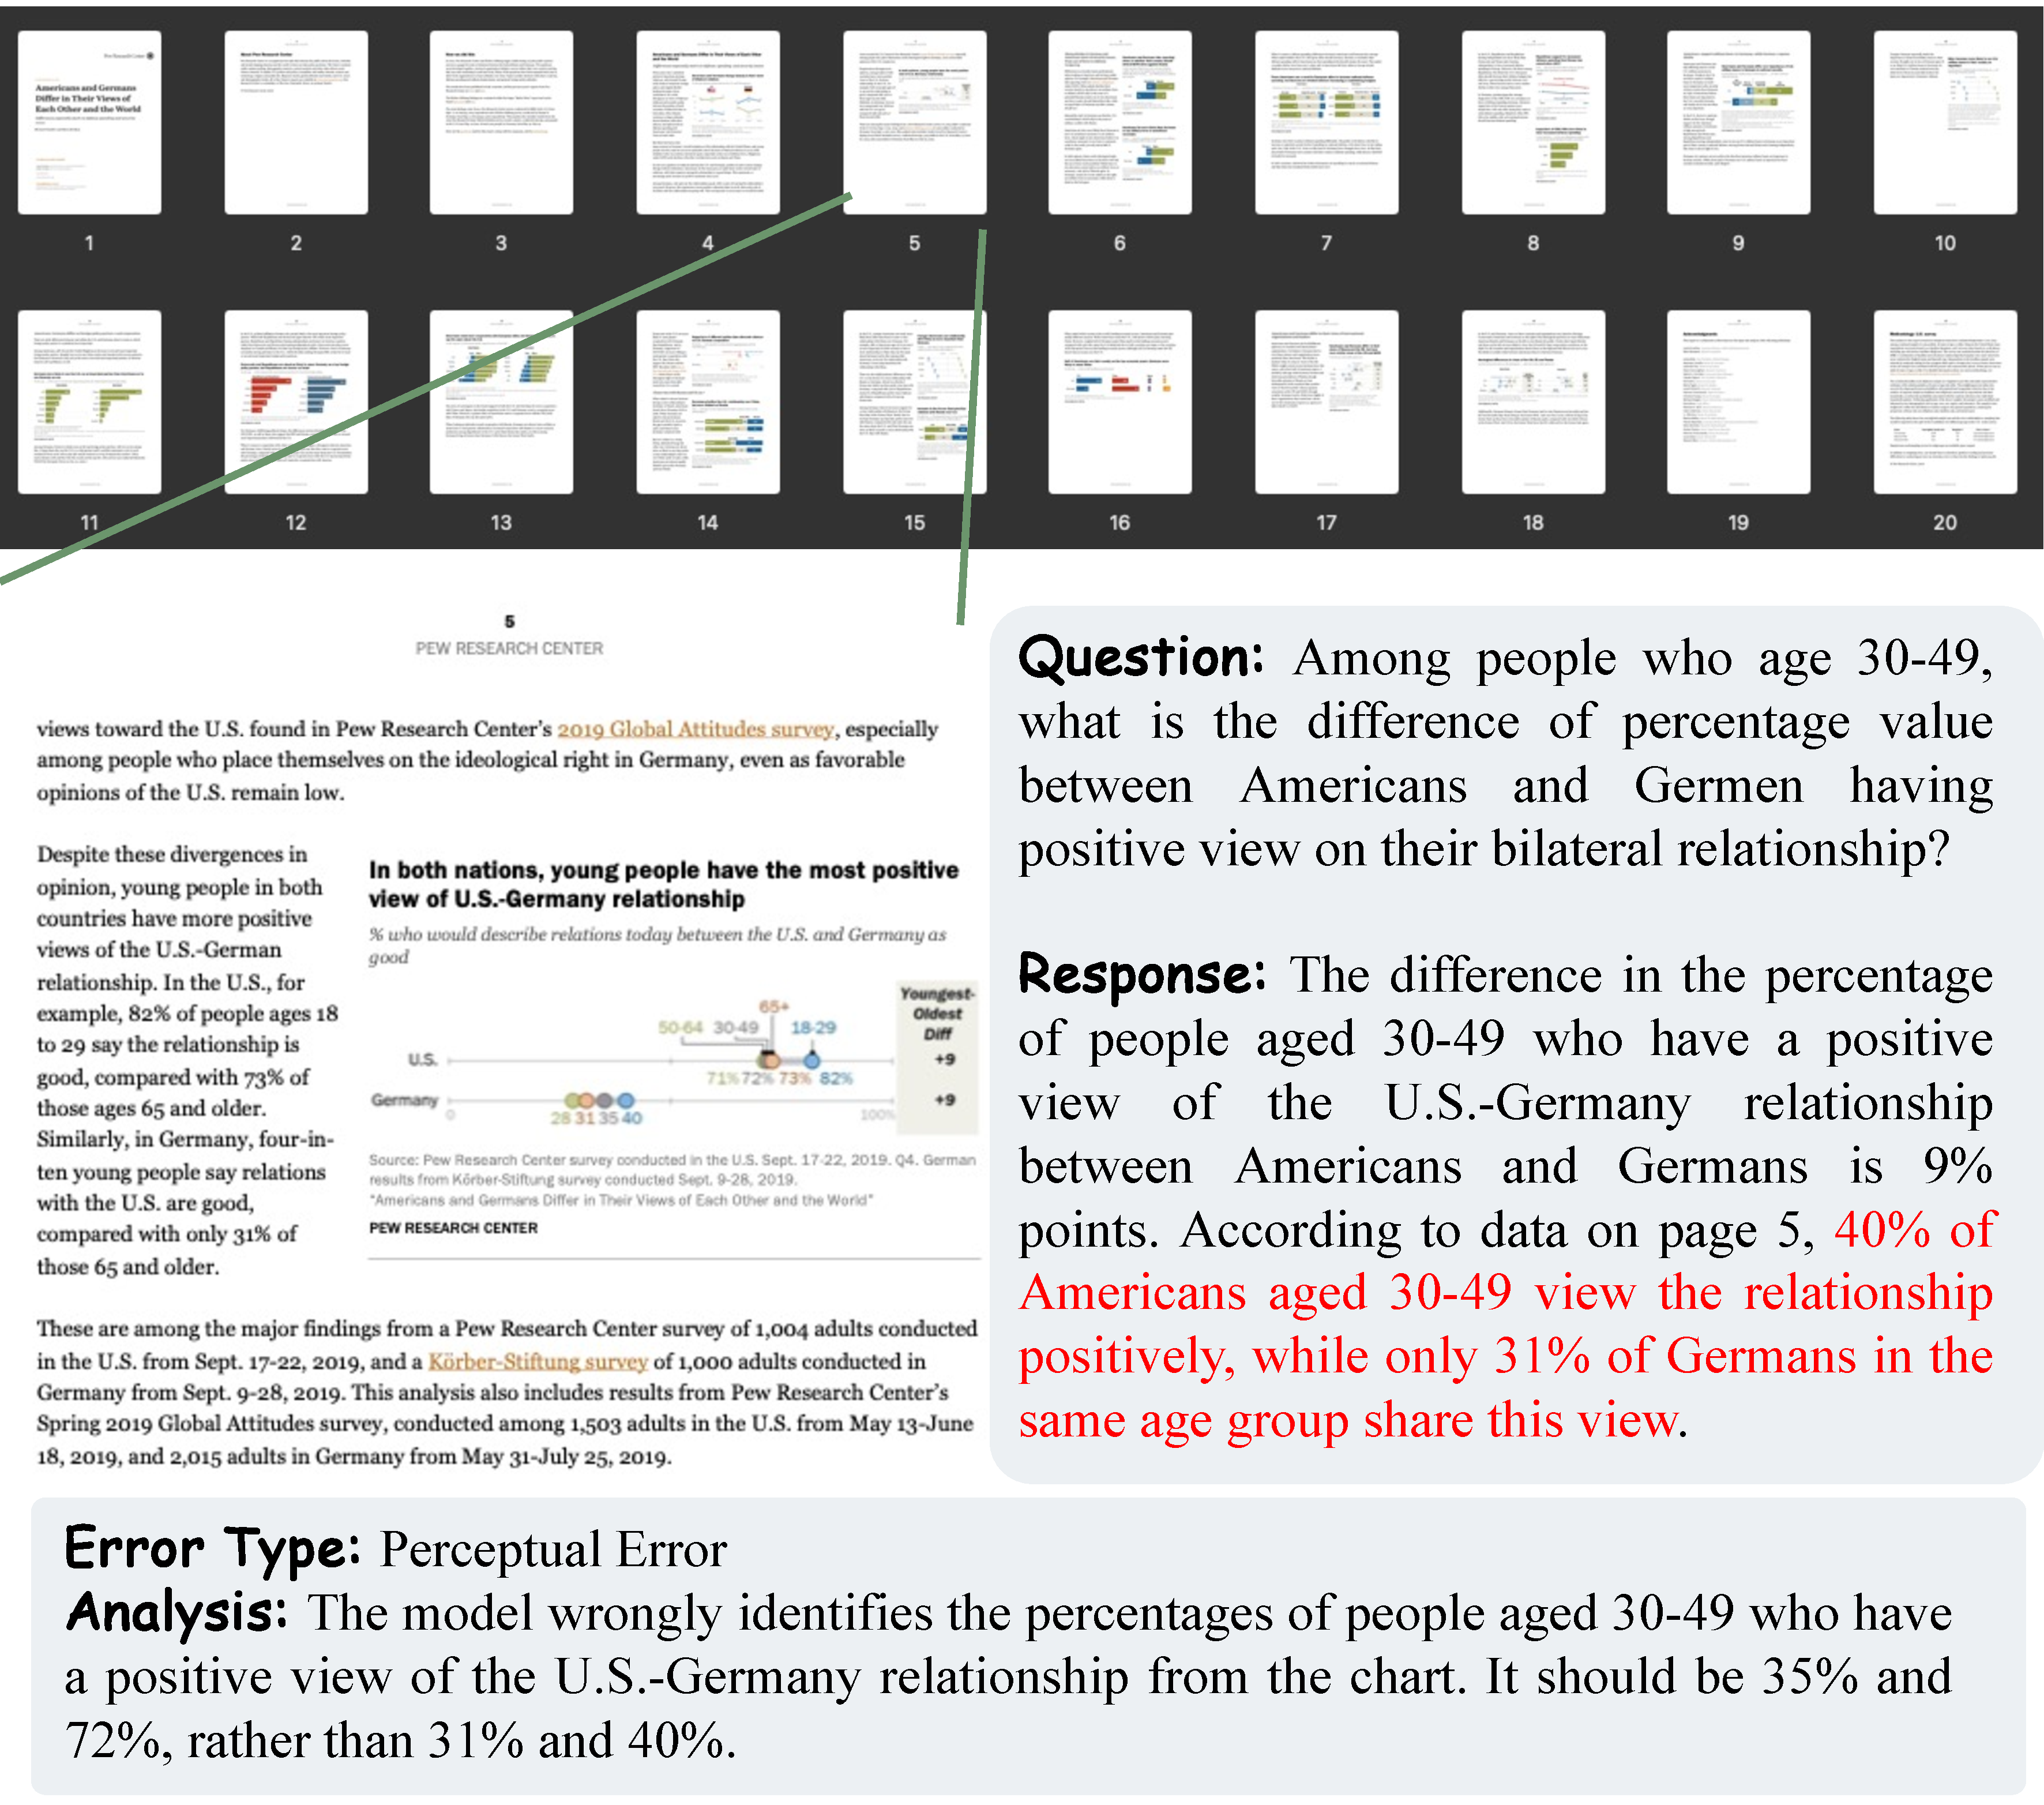
\includegraphics[width=\linewidth]{figures/Perceptual_error_1.pdf}
    \caption{Error example about \textit{Perceptual Error}}
    \label{fig: Perceptual_error_1}
\end{figure}

\clearpage
\noindent\textbf{Perceptual Error: Case 2}
\begin{figure}[!htbp]
    \centering
    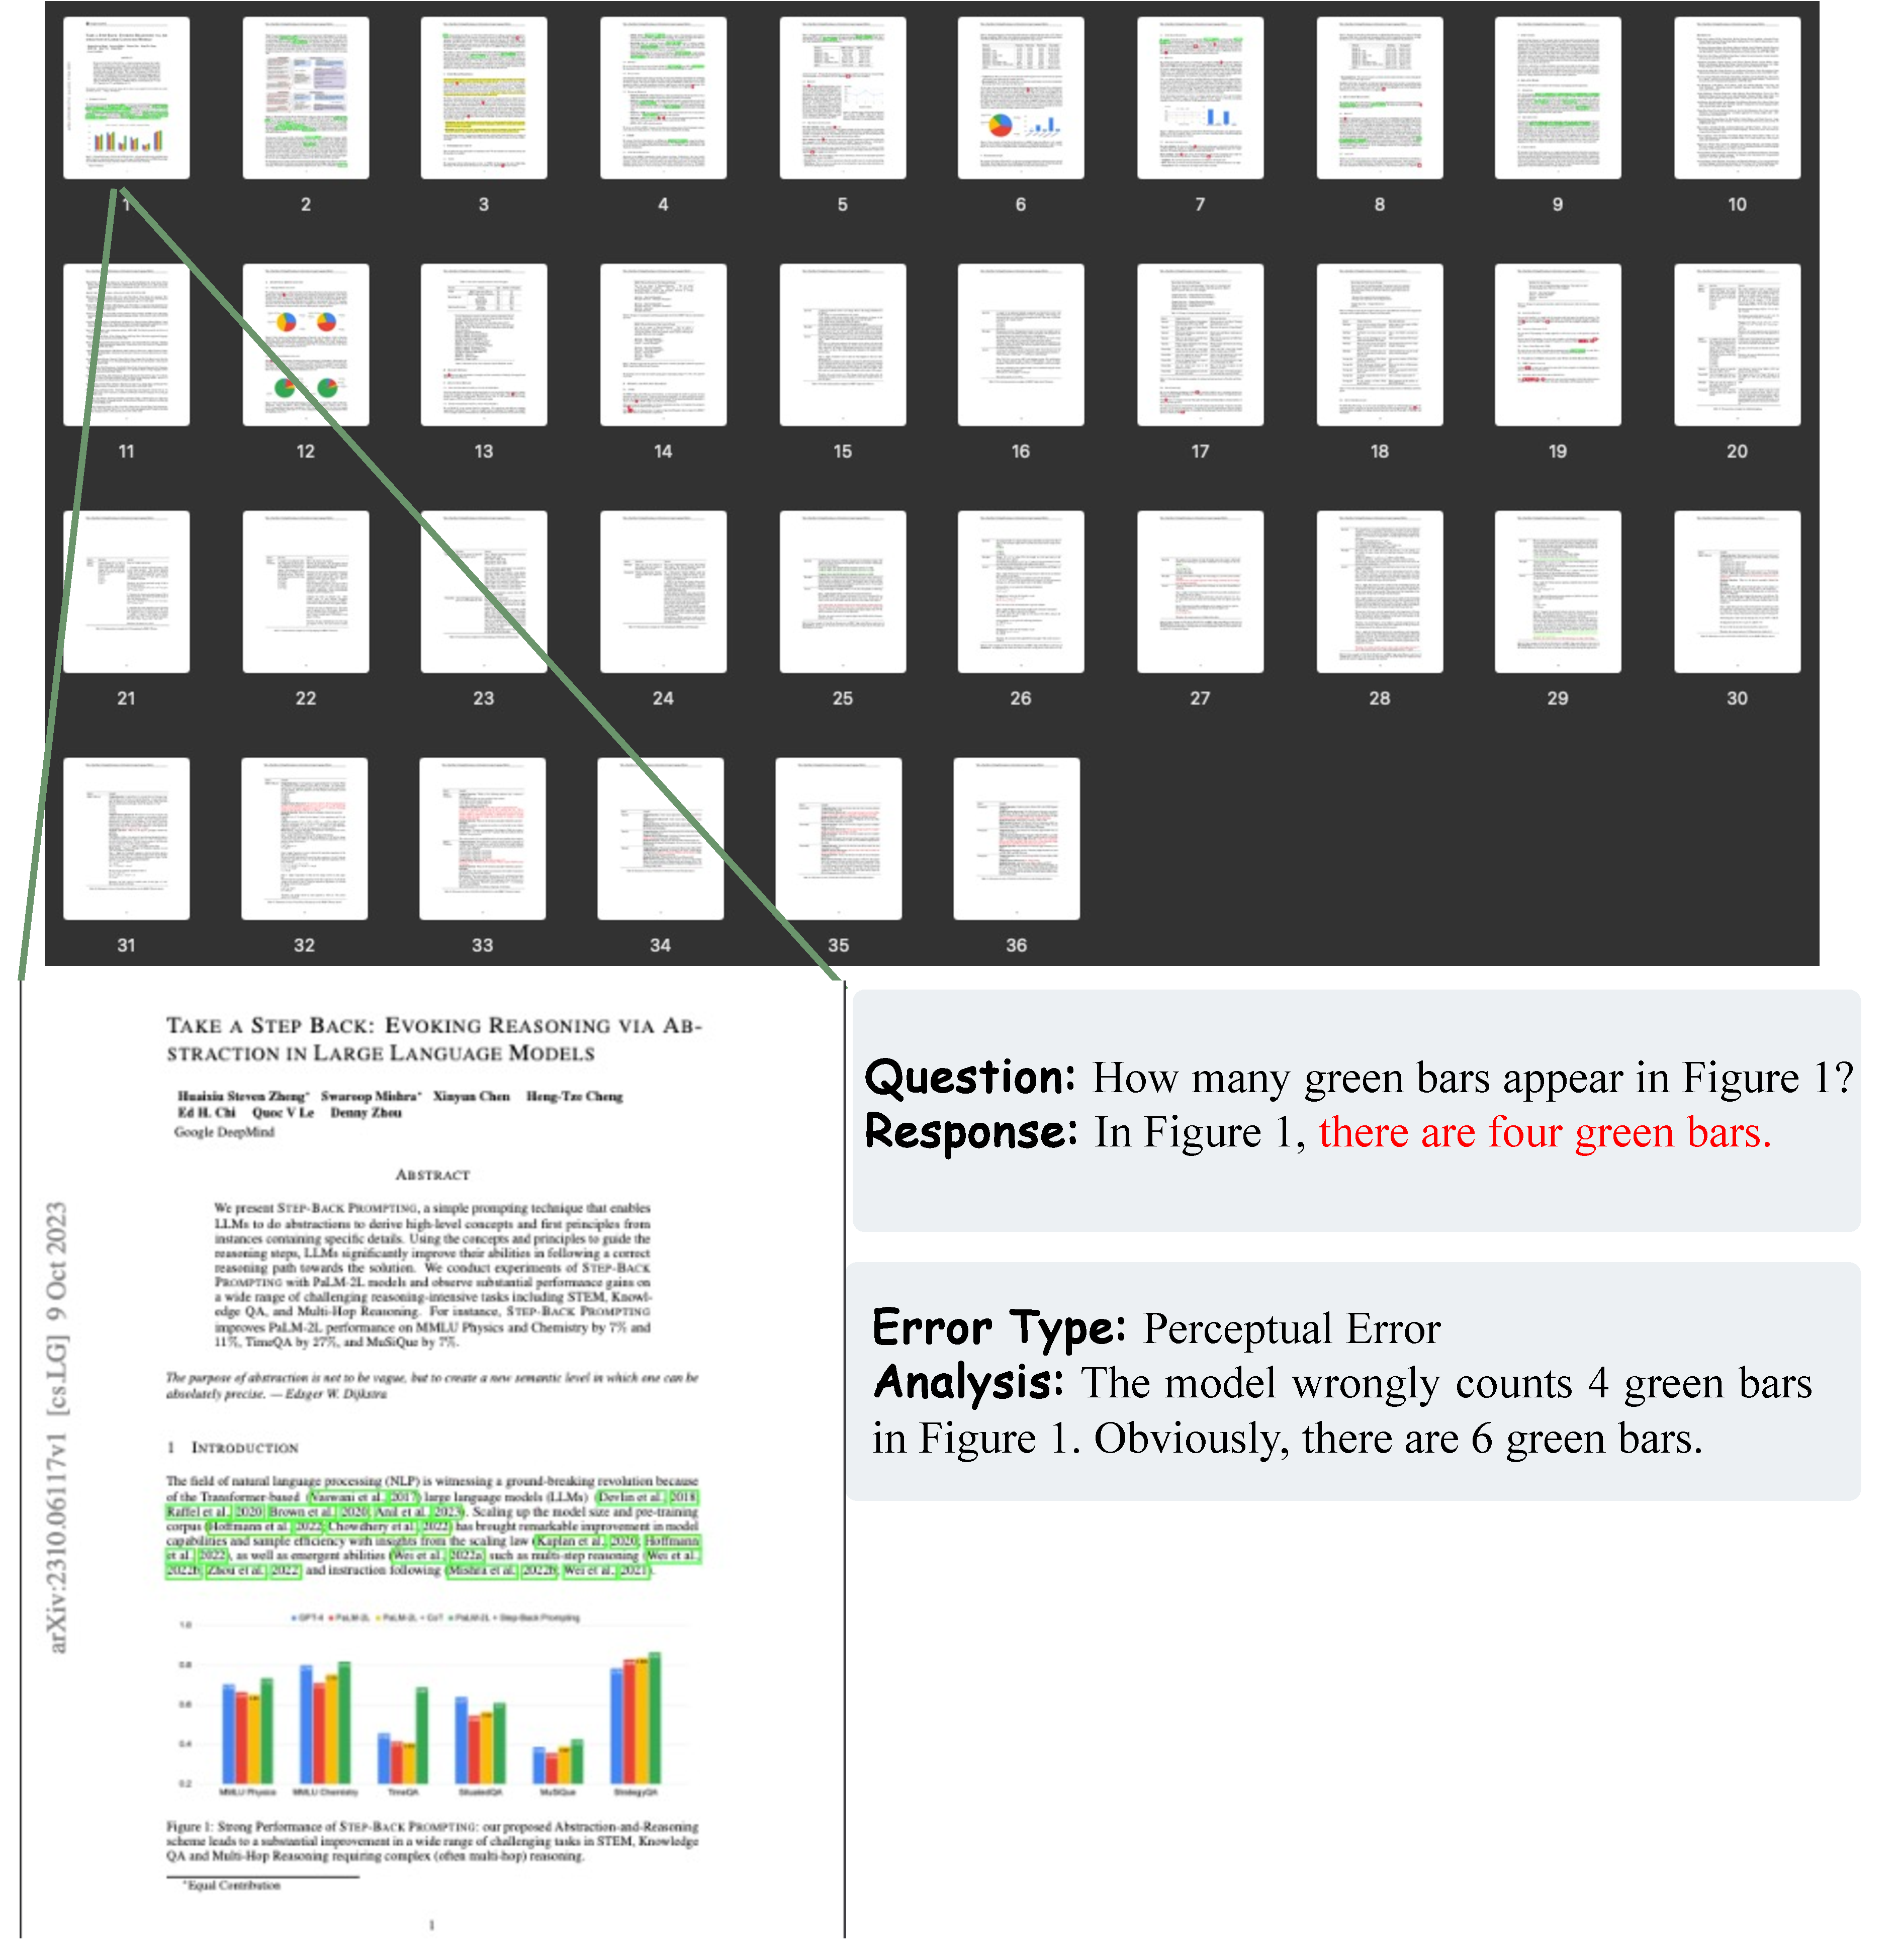
\includegraphics[width=\linewidth]{figures/Perceptual_error_2.pdf}
    \caption{Error example about \textit{Perceptual Error}}
    \label{fig: Perceptual_error_2}
\end{figure}

\clearpage
\noindent\textbf{Incomplete Evidence: Case 1}
\begin{figure}[!htbp]
    \centering
    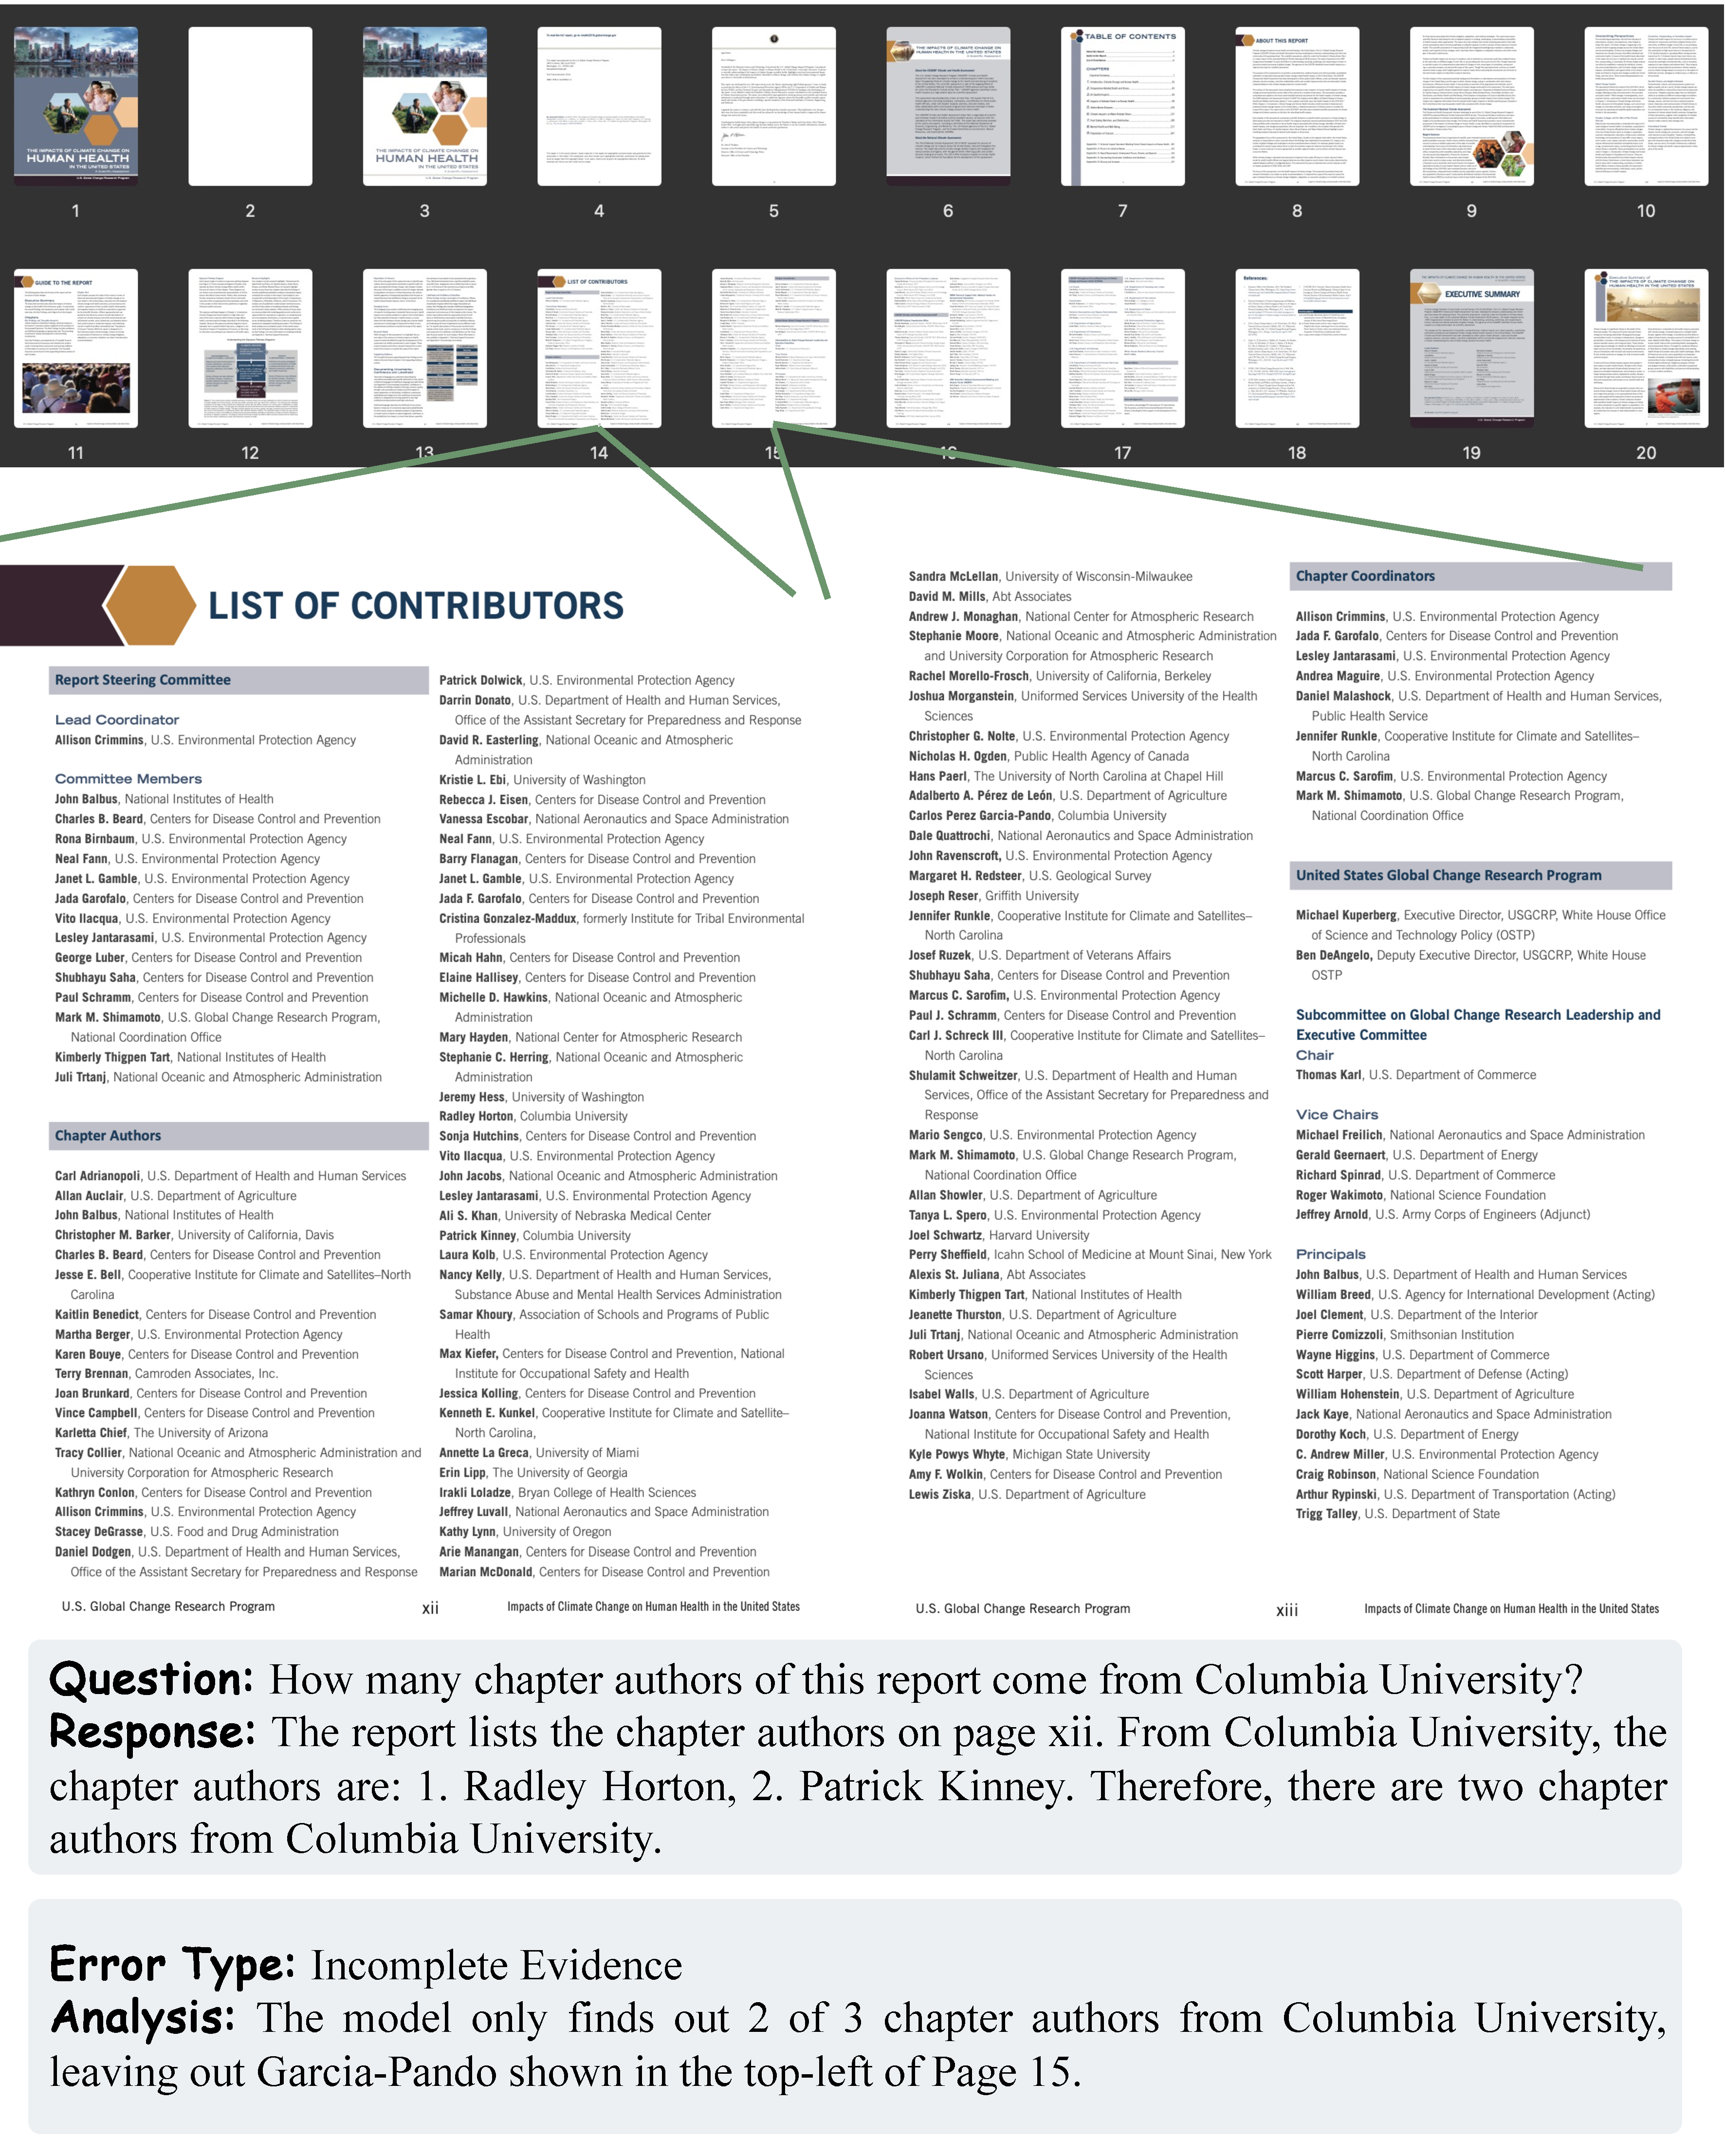
\includegraphics[width=\linewidth]{figures/Incomplete_evidence.pdf}
    \caption{Error example about \textit{Incomplete Evidence}}
    \label{fig: Incomplete_evidence_1}
\end{figure}

\clearpage
\noindent\textbf{Incomplete Evidence: Case 2}
\begin{figure}[!htbp]
    \centering
    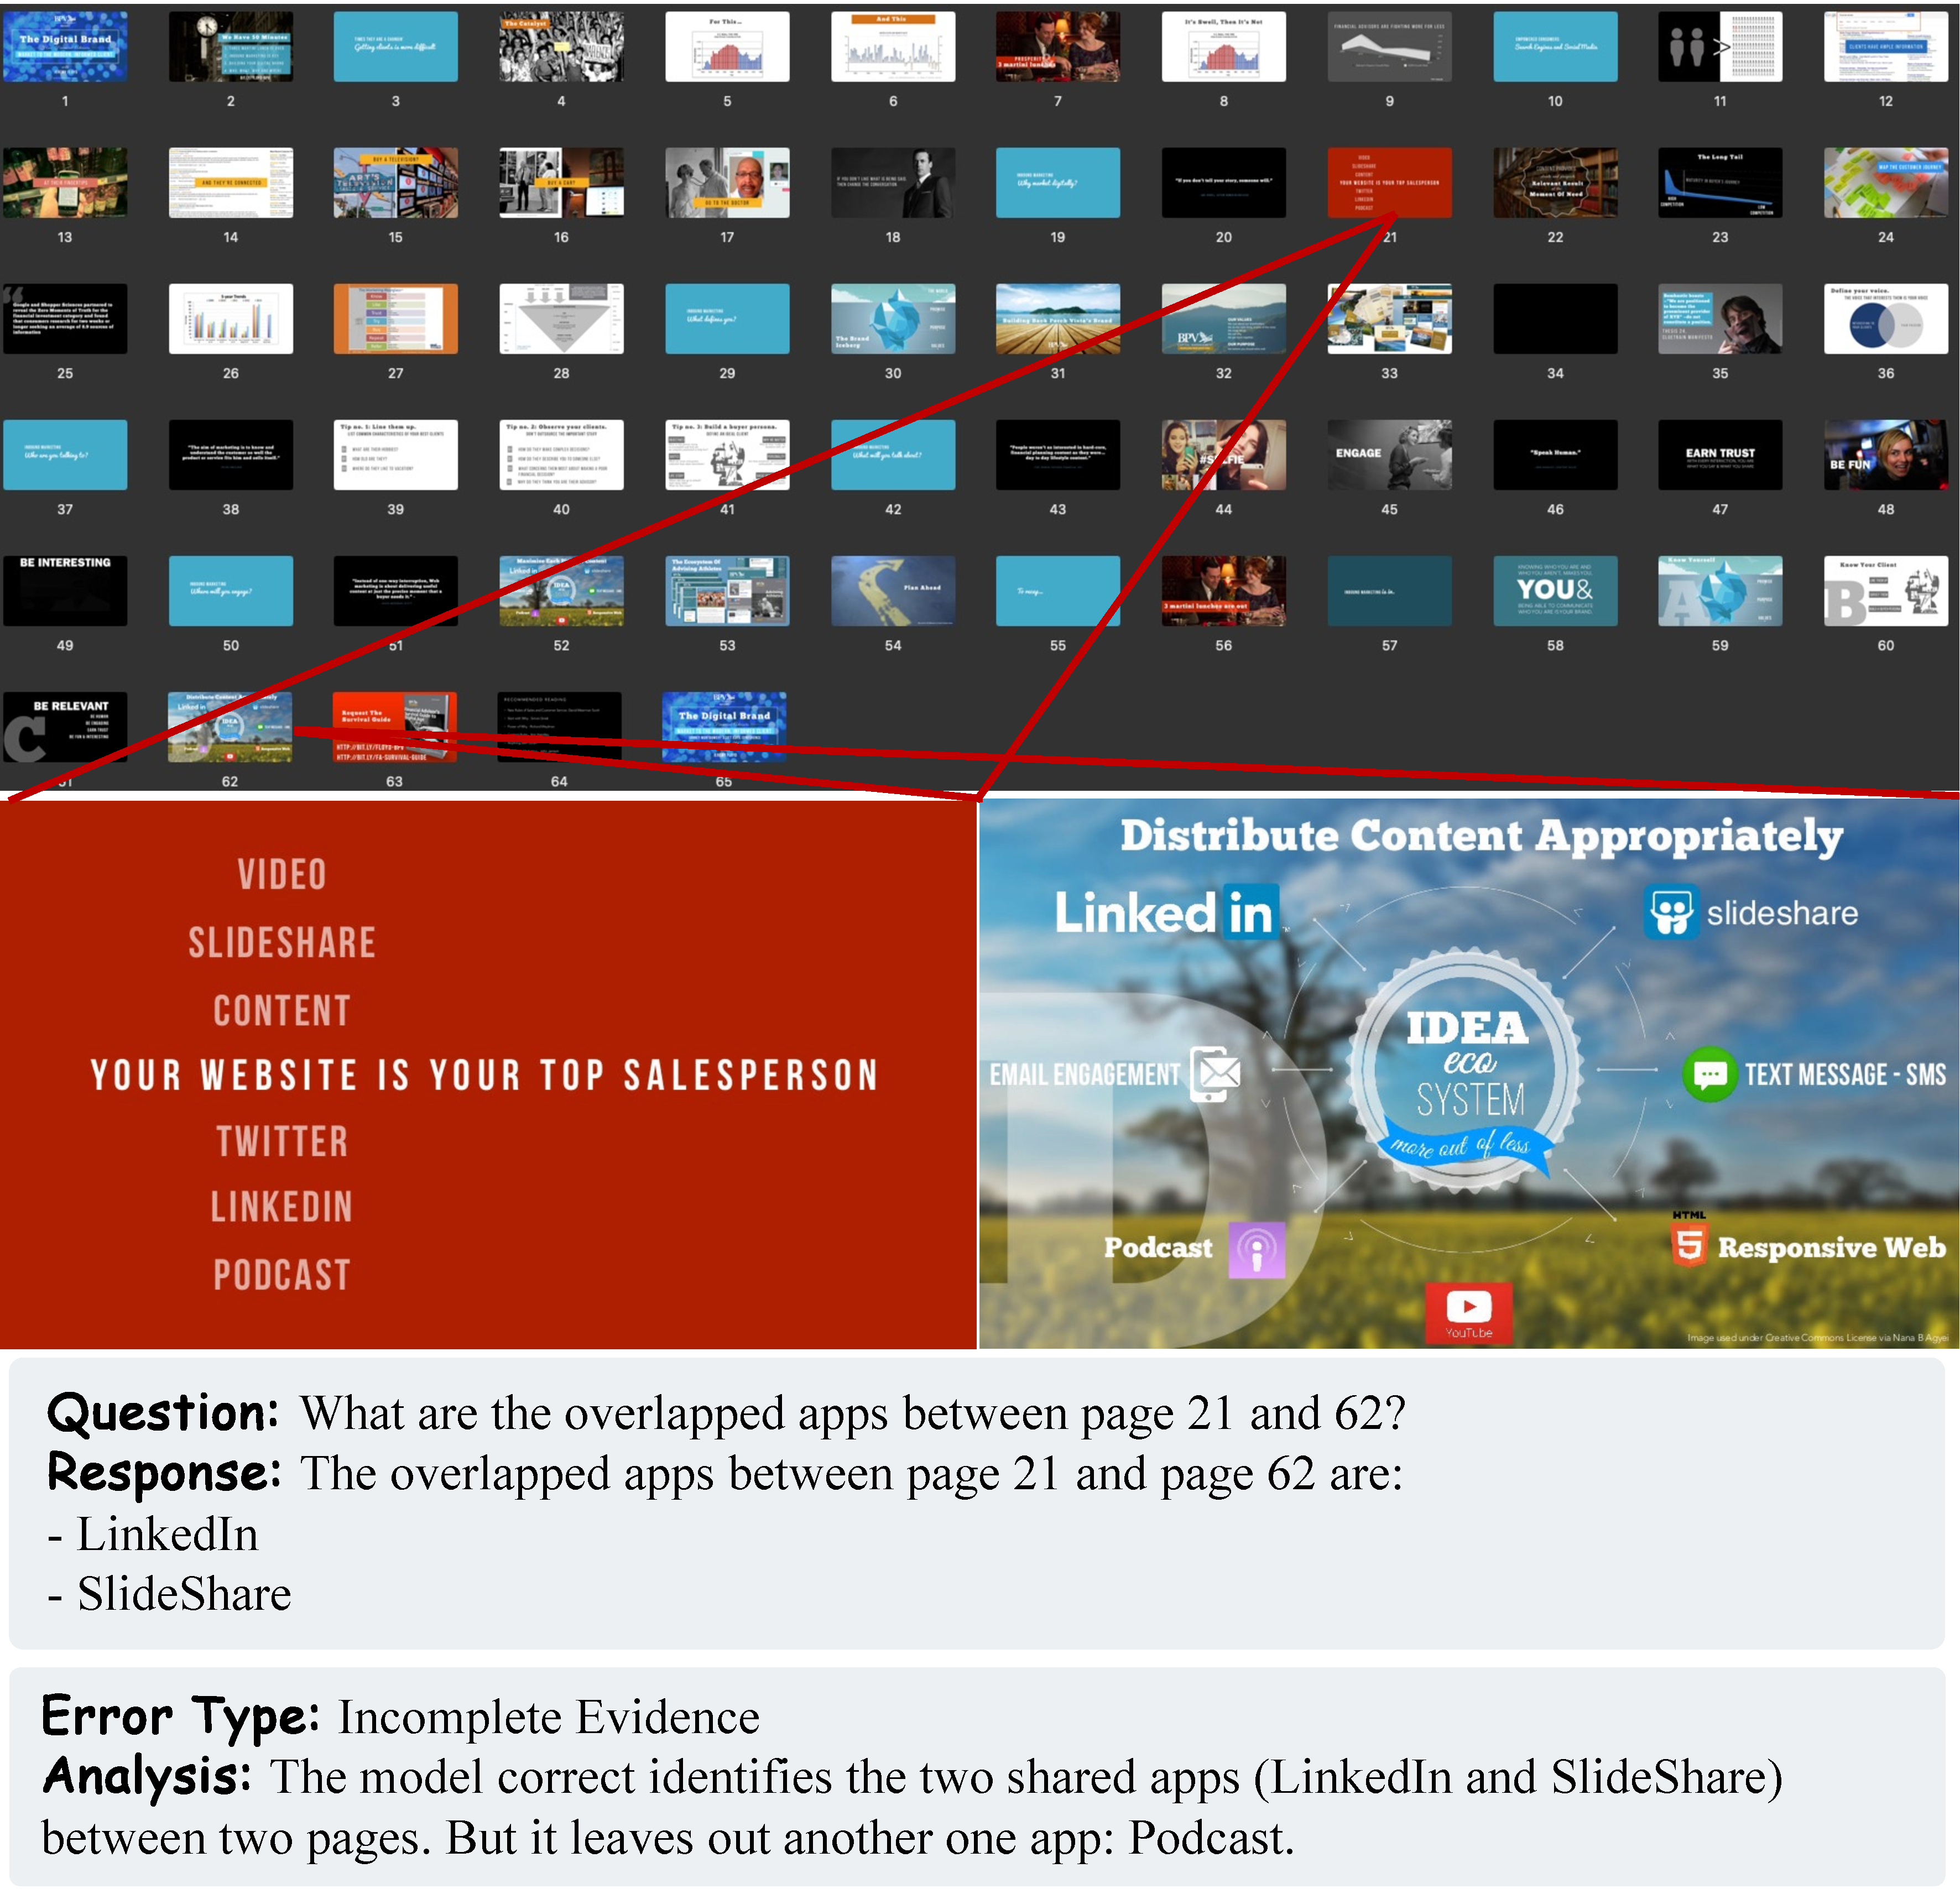
\includegraphics[width=\linewidth]{figures/Incomplete_evidence_2.pdf}
    \caption{Error example about \textit{Incomplete Evidence}}
    \label{fig: Incomplete_evidence_2}
\end{figure}

\clearpage
\noindent\textbf{Hallucinated Evidence: Case 1}
\begin{figure}[!htbp]
    \centering
    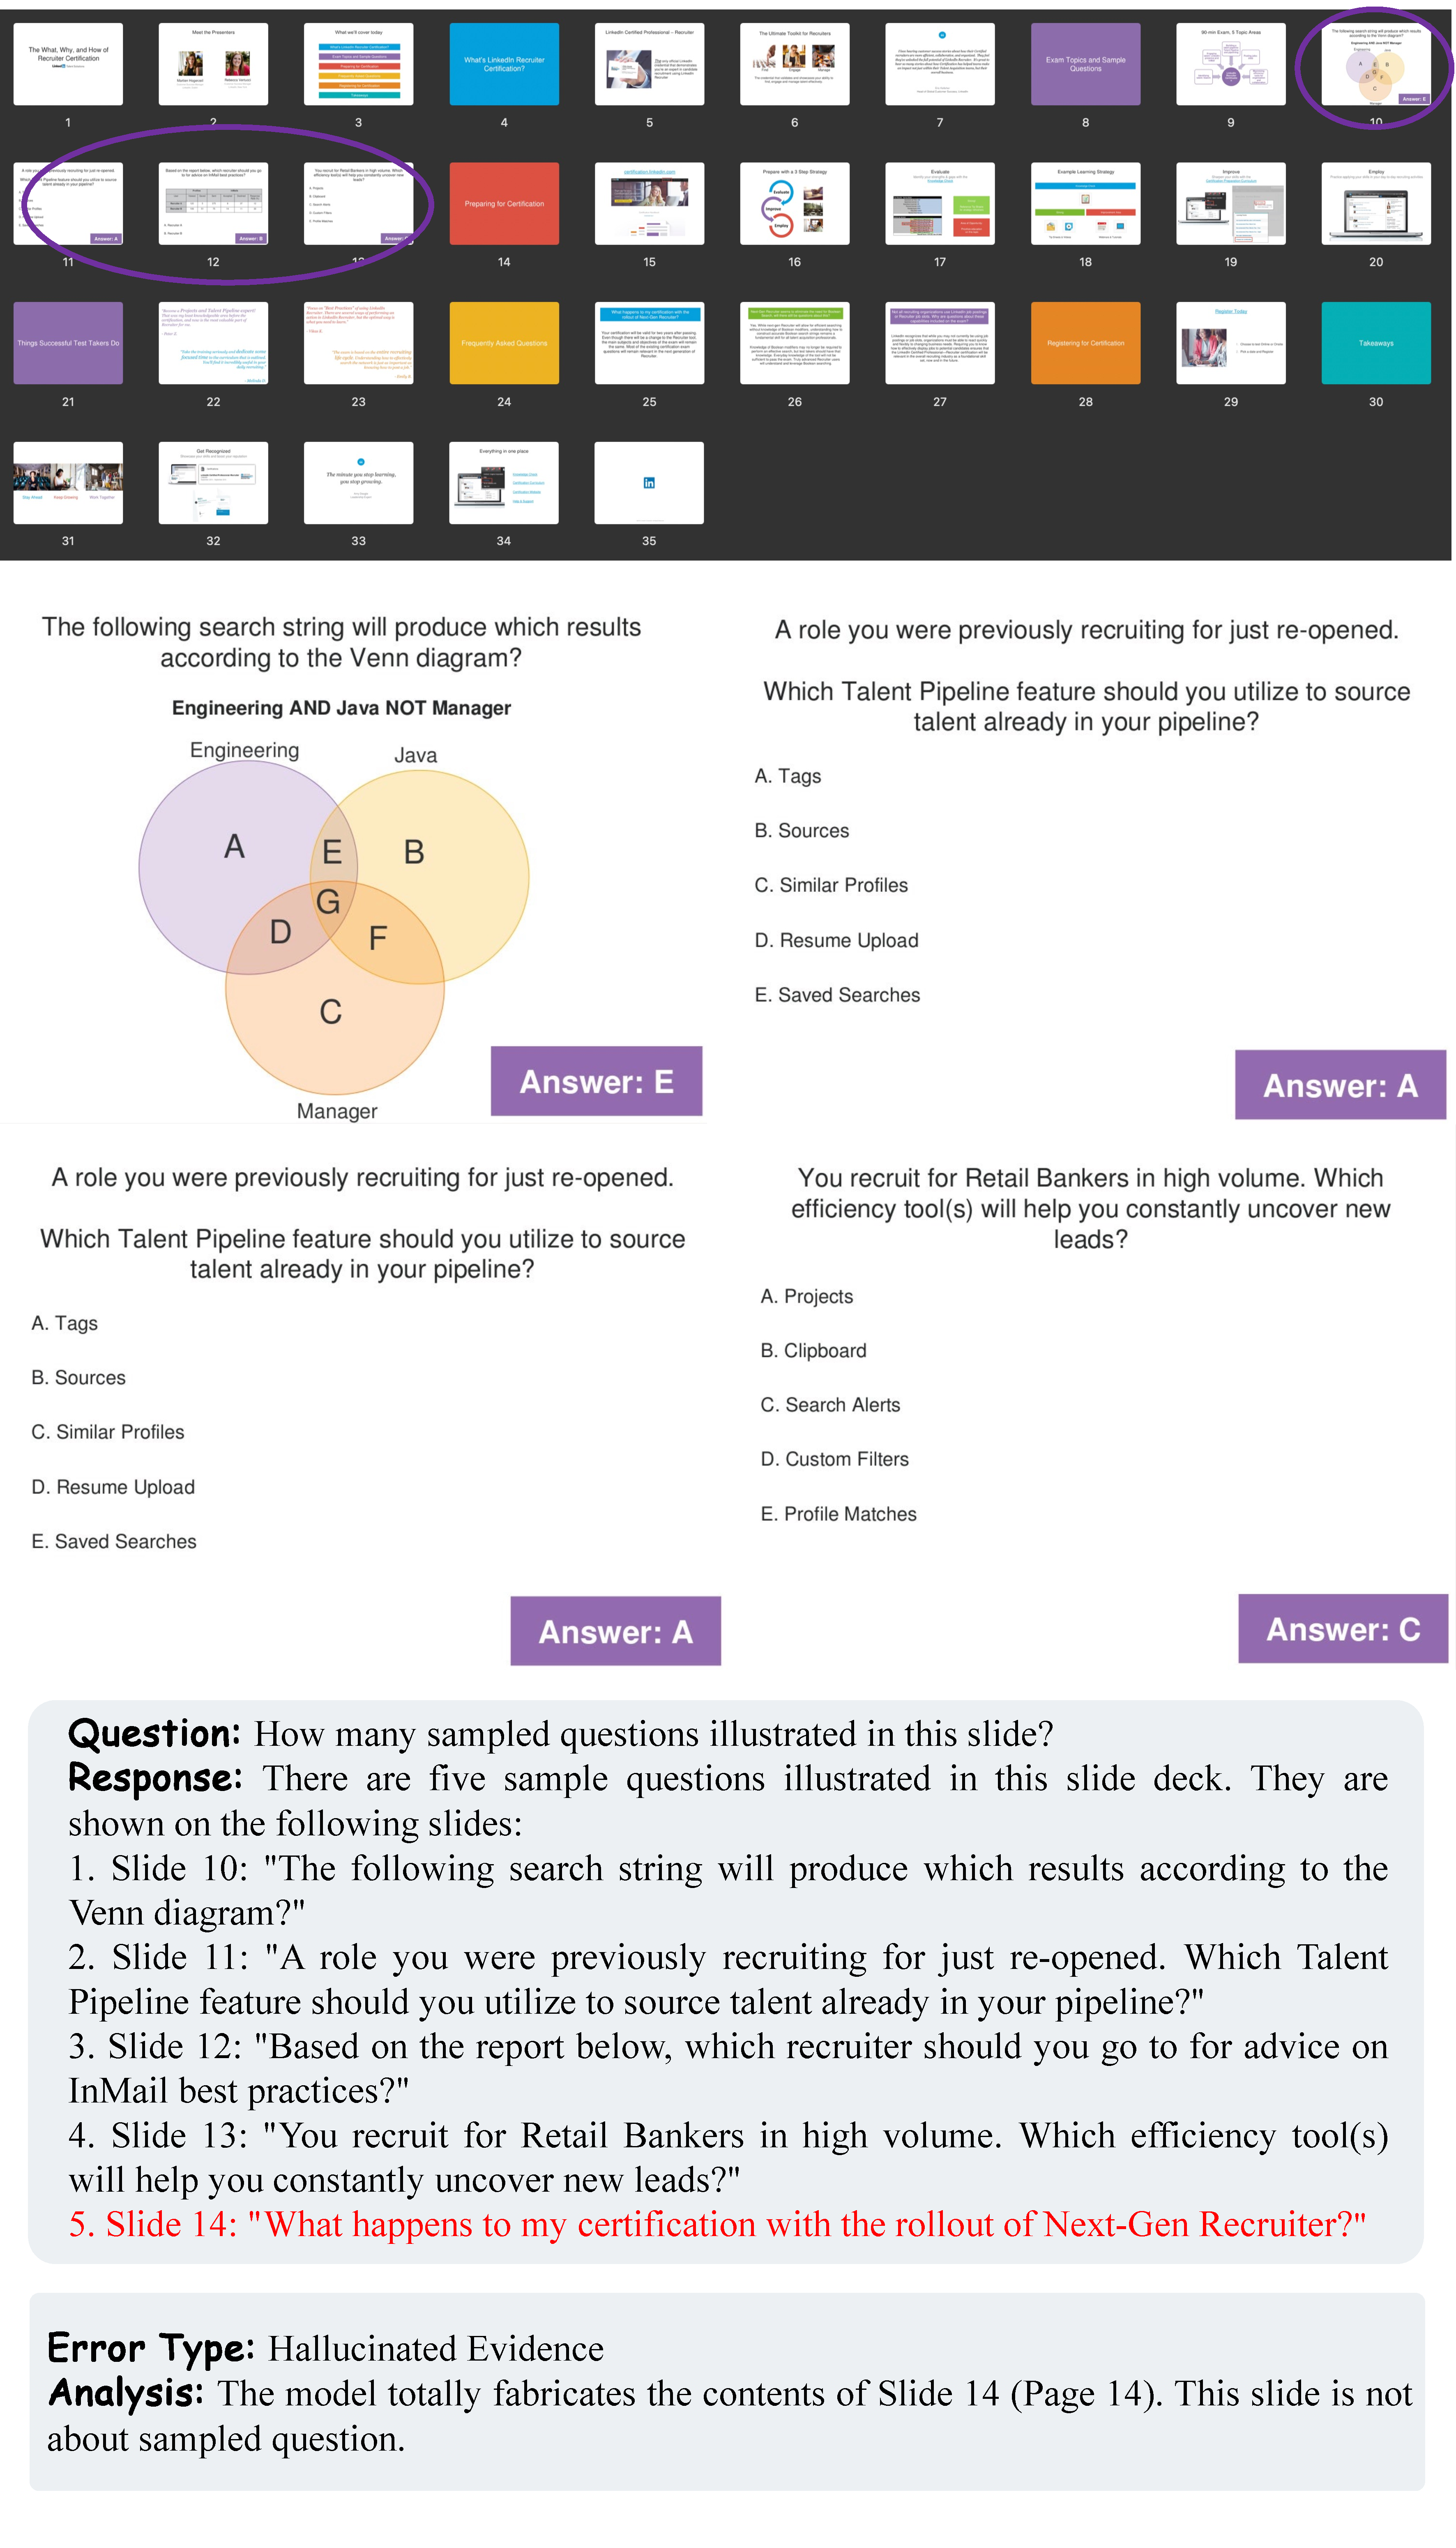
\includegraphics[width=0.85\linewidth]{figures/Hallucinated_error.pdf}
    \caption{Error example about \textit{Hallucinated Evidence}}
    \label{fig: Hallucinated_evidence_1}
\end{figure}

\clearpage
\noindent\textbf{Hallucinated Evidence: Case 2}
\begin{figure}[!htbp]
    \centering
    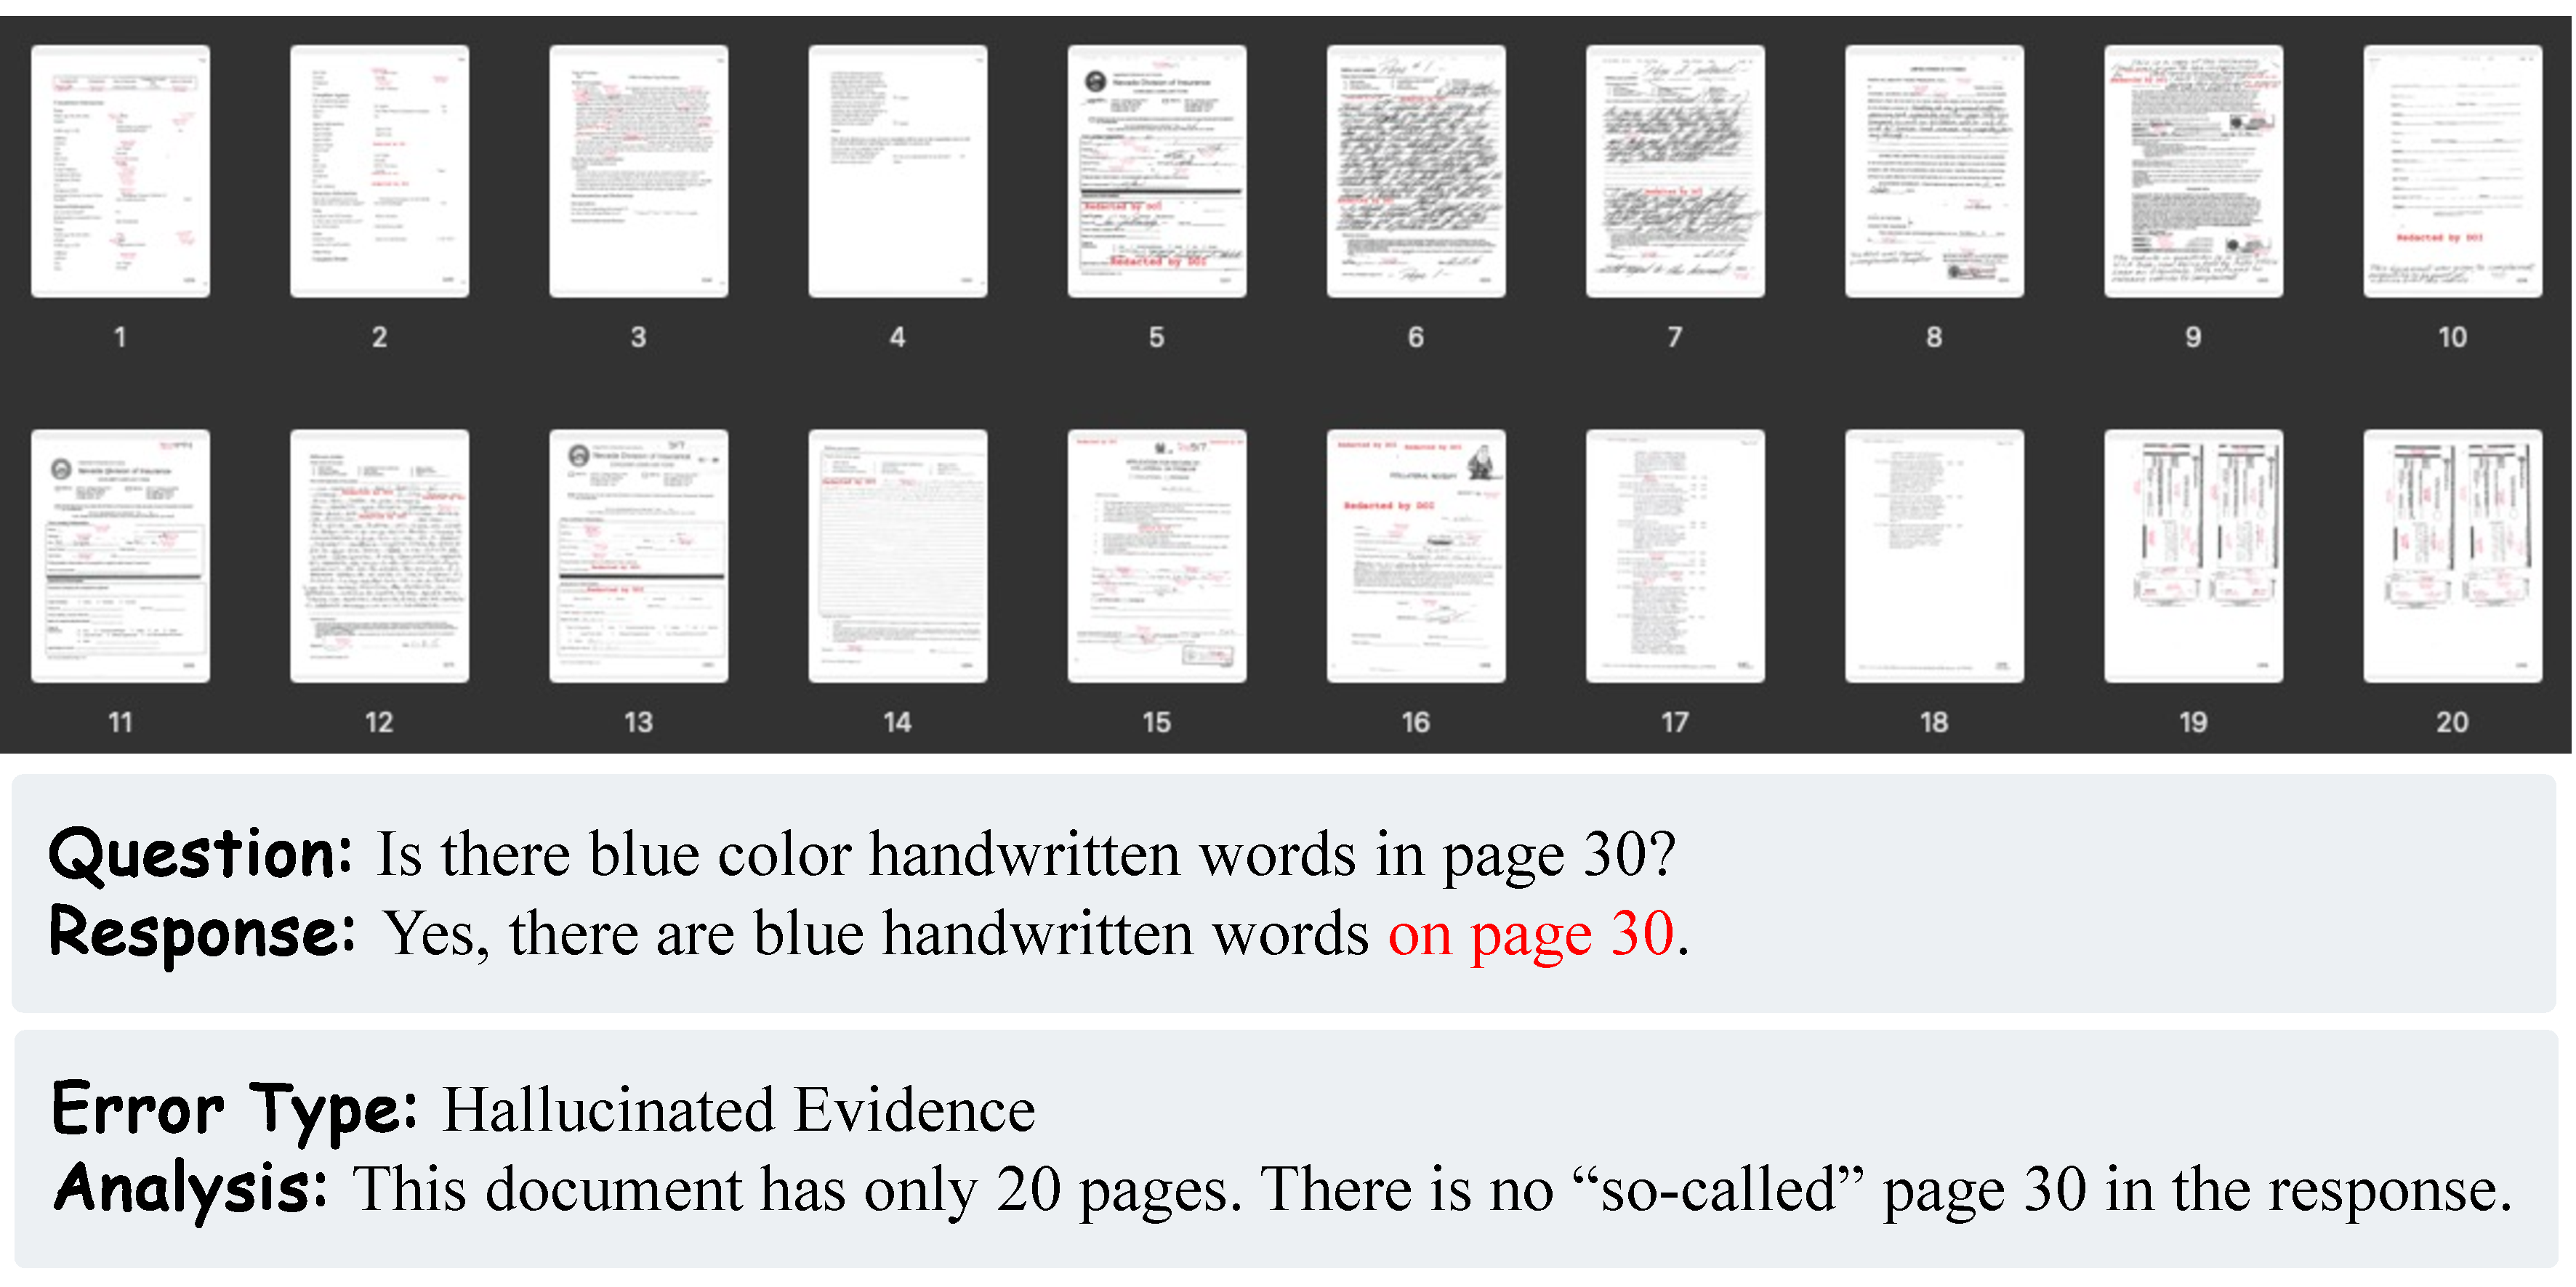
\includegraphics[width=0.85\linewidth]{figures/Halllucinated_error_2.pdf}
    \caption{Error example about \textit{Hallucinated Evidence}}
    \label{fig: Hallucinated_evidence_2}
\end{figure}

\clearpage
\noindent\textbf{Knowledge Lacking: Case 1}
\begin{figure}[!htbp]
    \centering
    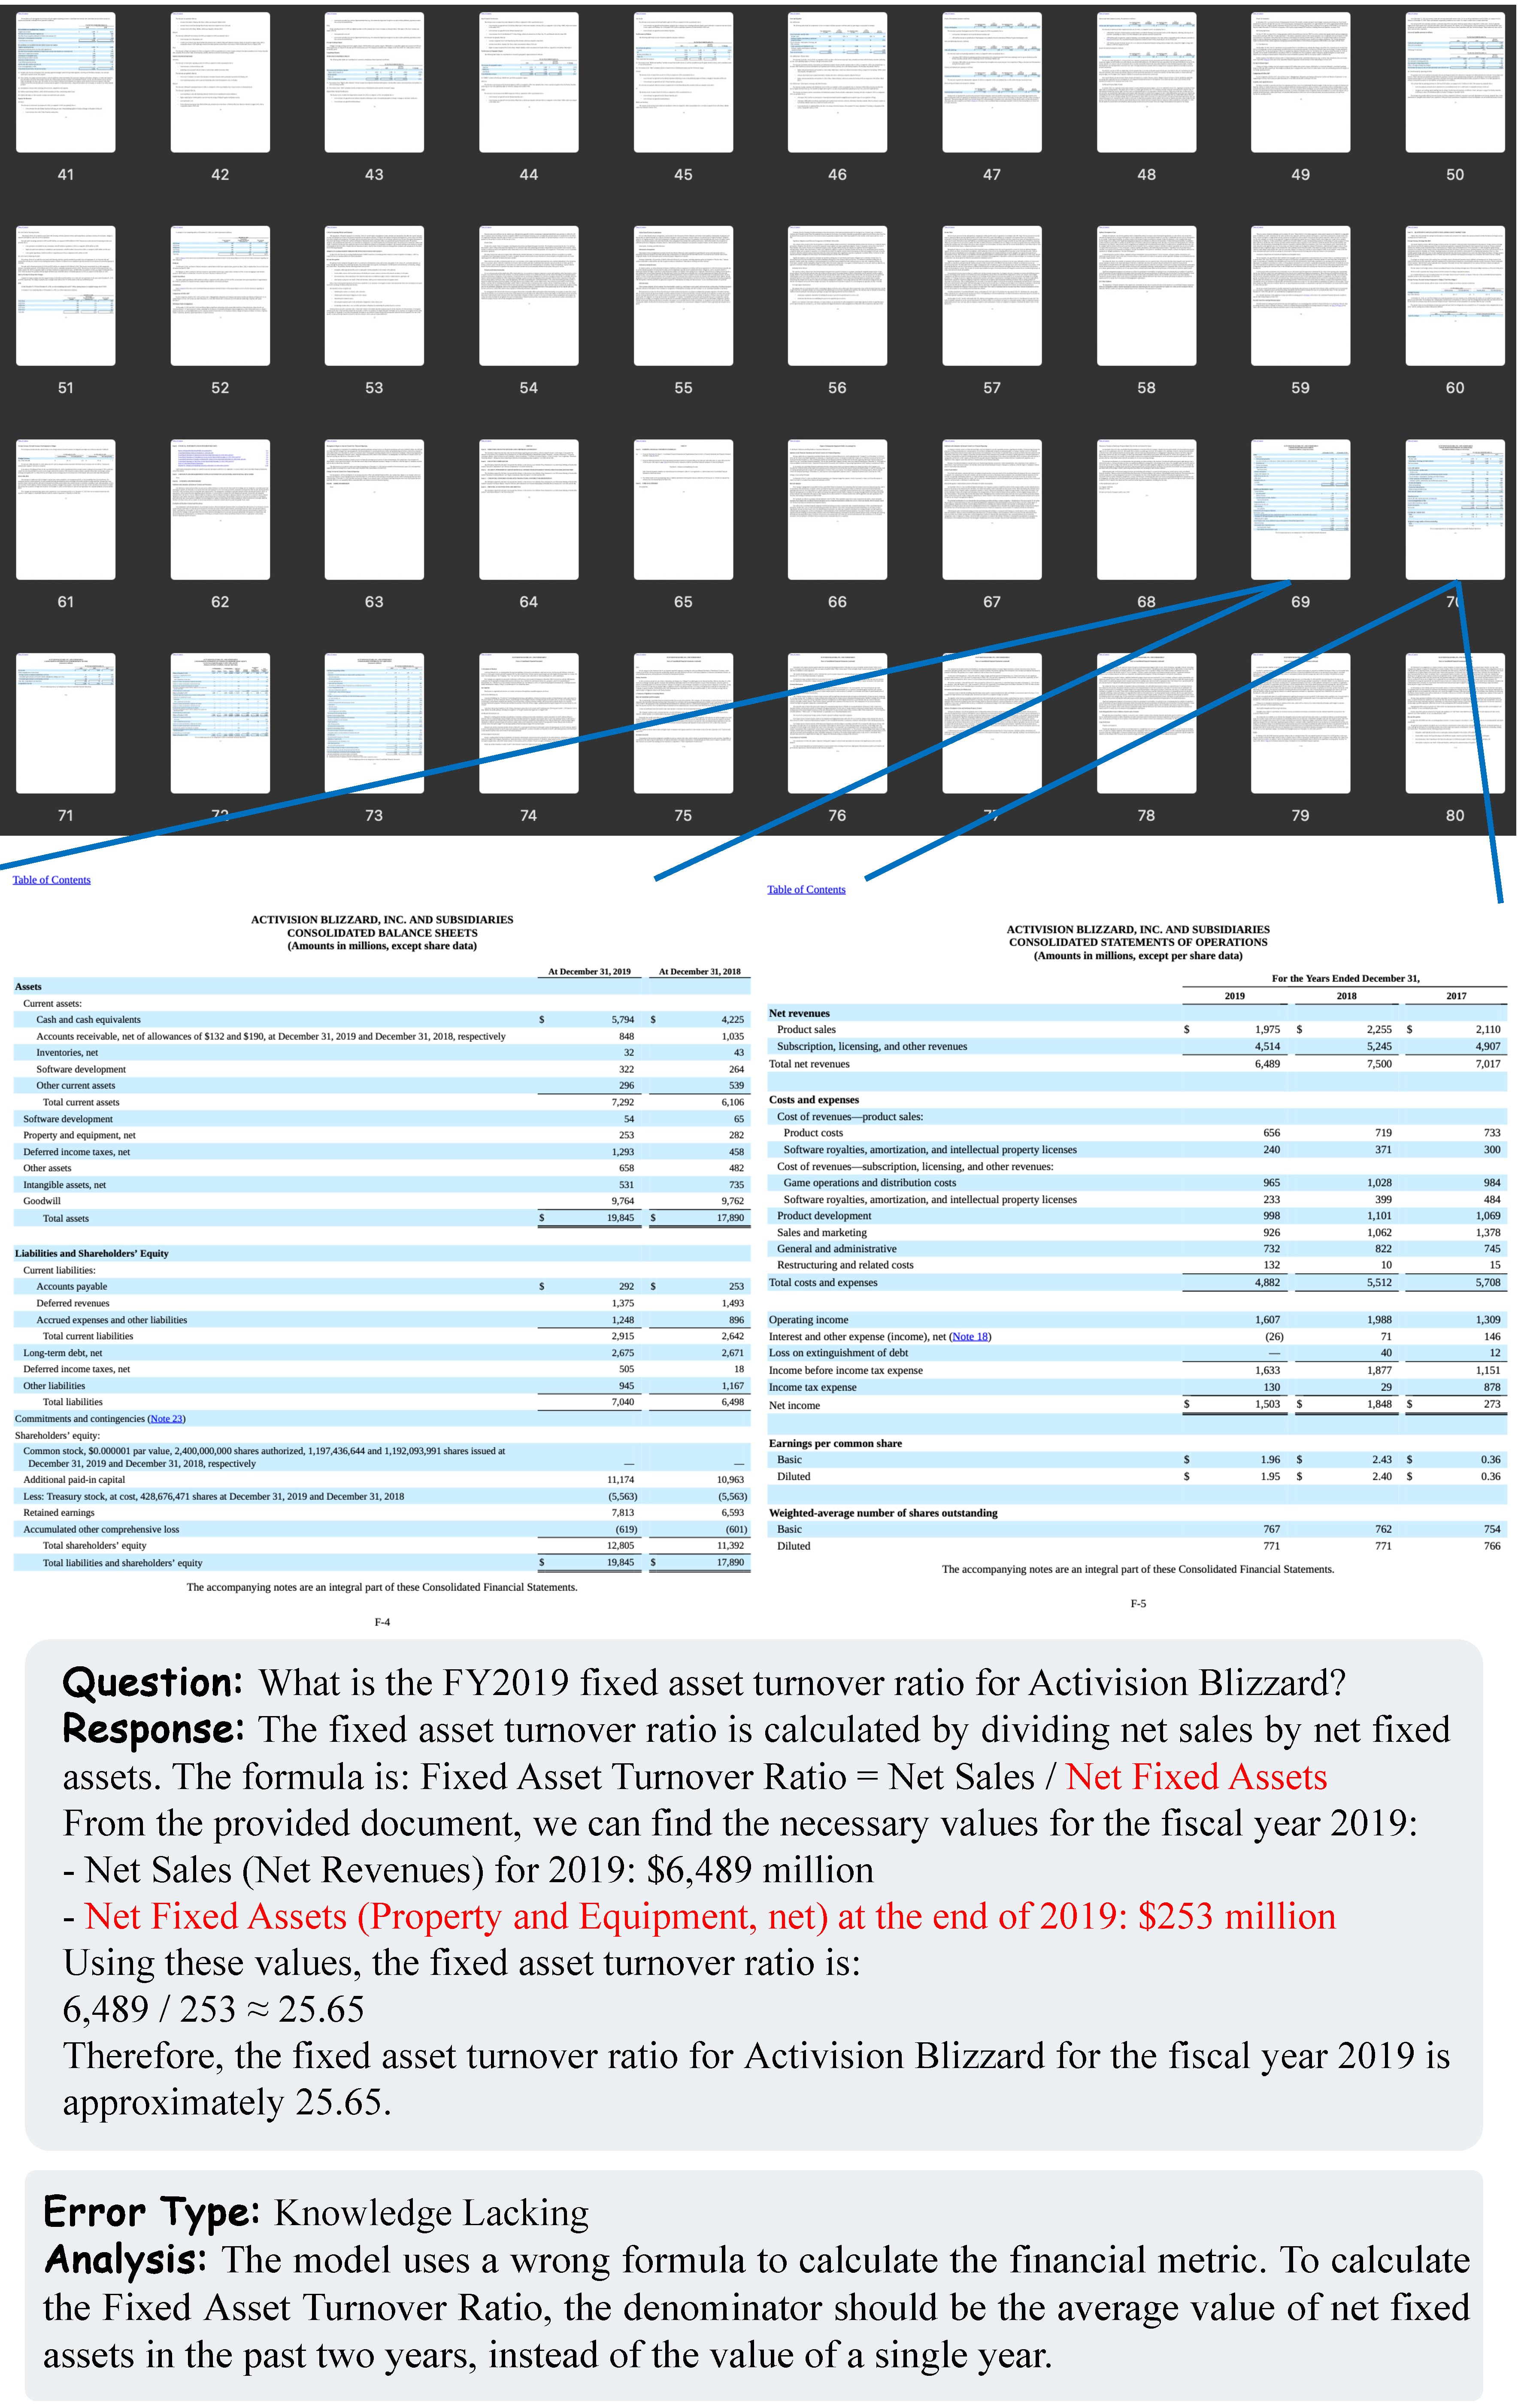
\includegraphics[width=0.95\linewidth]{figures/knowledge_lacking.pdf}
    \caption{Error example about \textit{Knowledge Lacking}}
    \label{fig: Knowledge_lacking_1}
\end{figure}

\clearpage
\noindent\textbf{Knowledge Lacking: Case 2}
\begin{figure}[!htbp]
    \centering
    \includegraphics[width=0.95\linewidth]{figures/knowledge_lacking_2.pdf}
    \caption{Error example about \textit{Knowledge Lacking}}
    \label{fig: Knowledge_lacking_2}
\end{figure}

\clearpage
\noindent\textbf{Reasoning Error: Case 1}
\begin{figure}[!htbp]
    \centering
    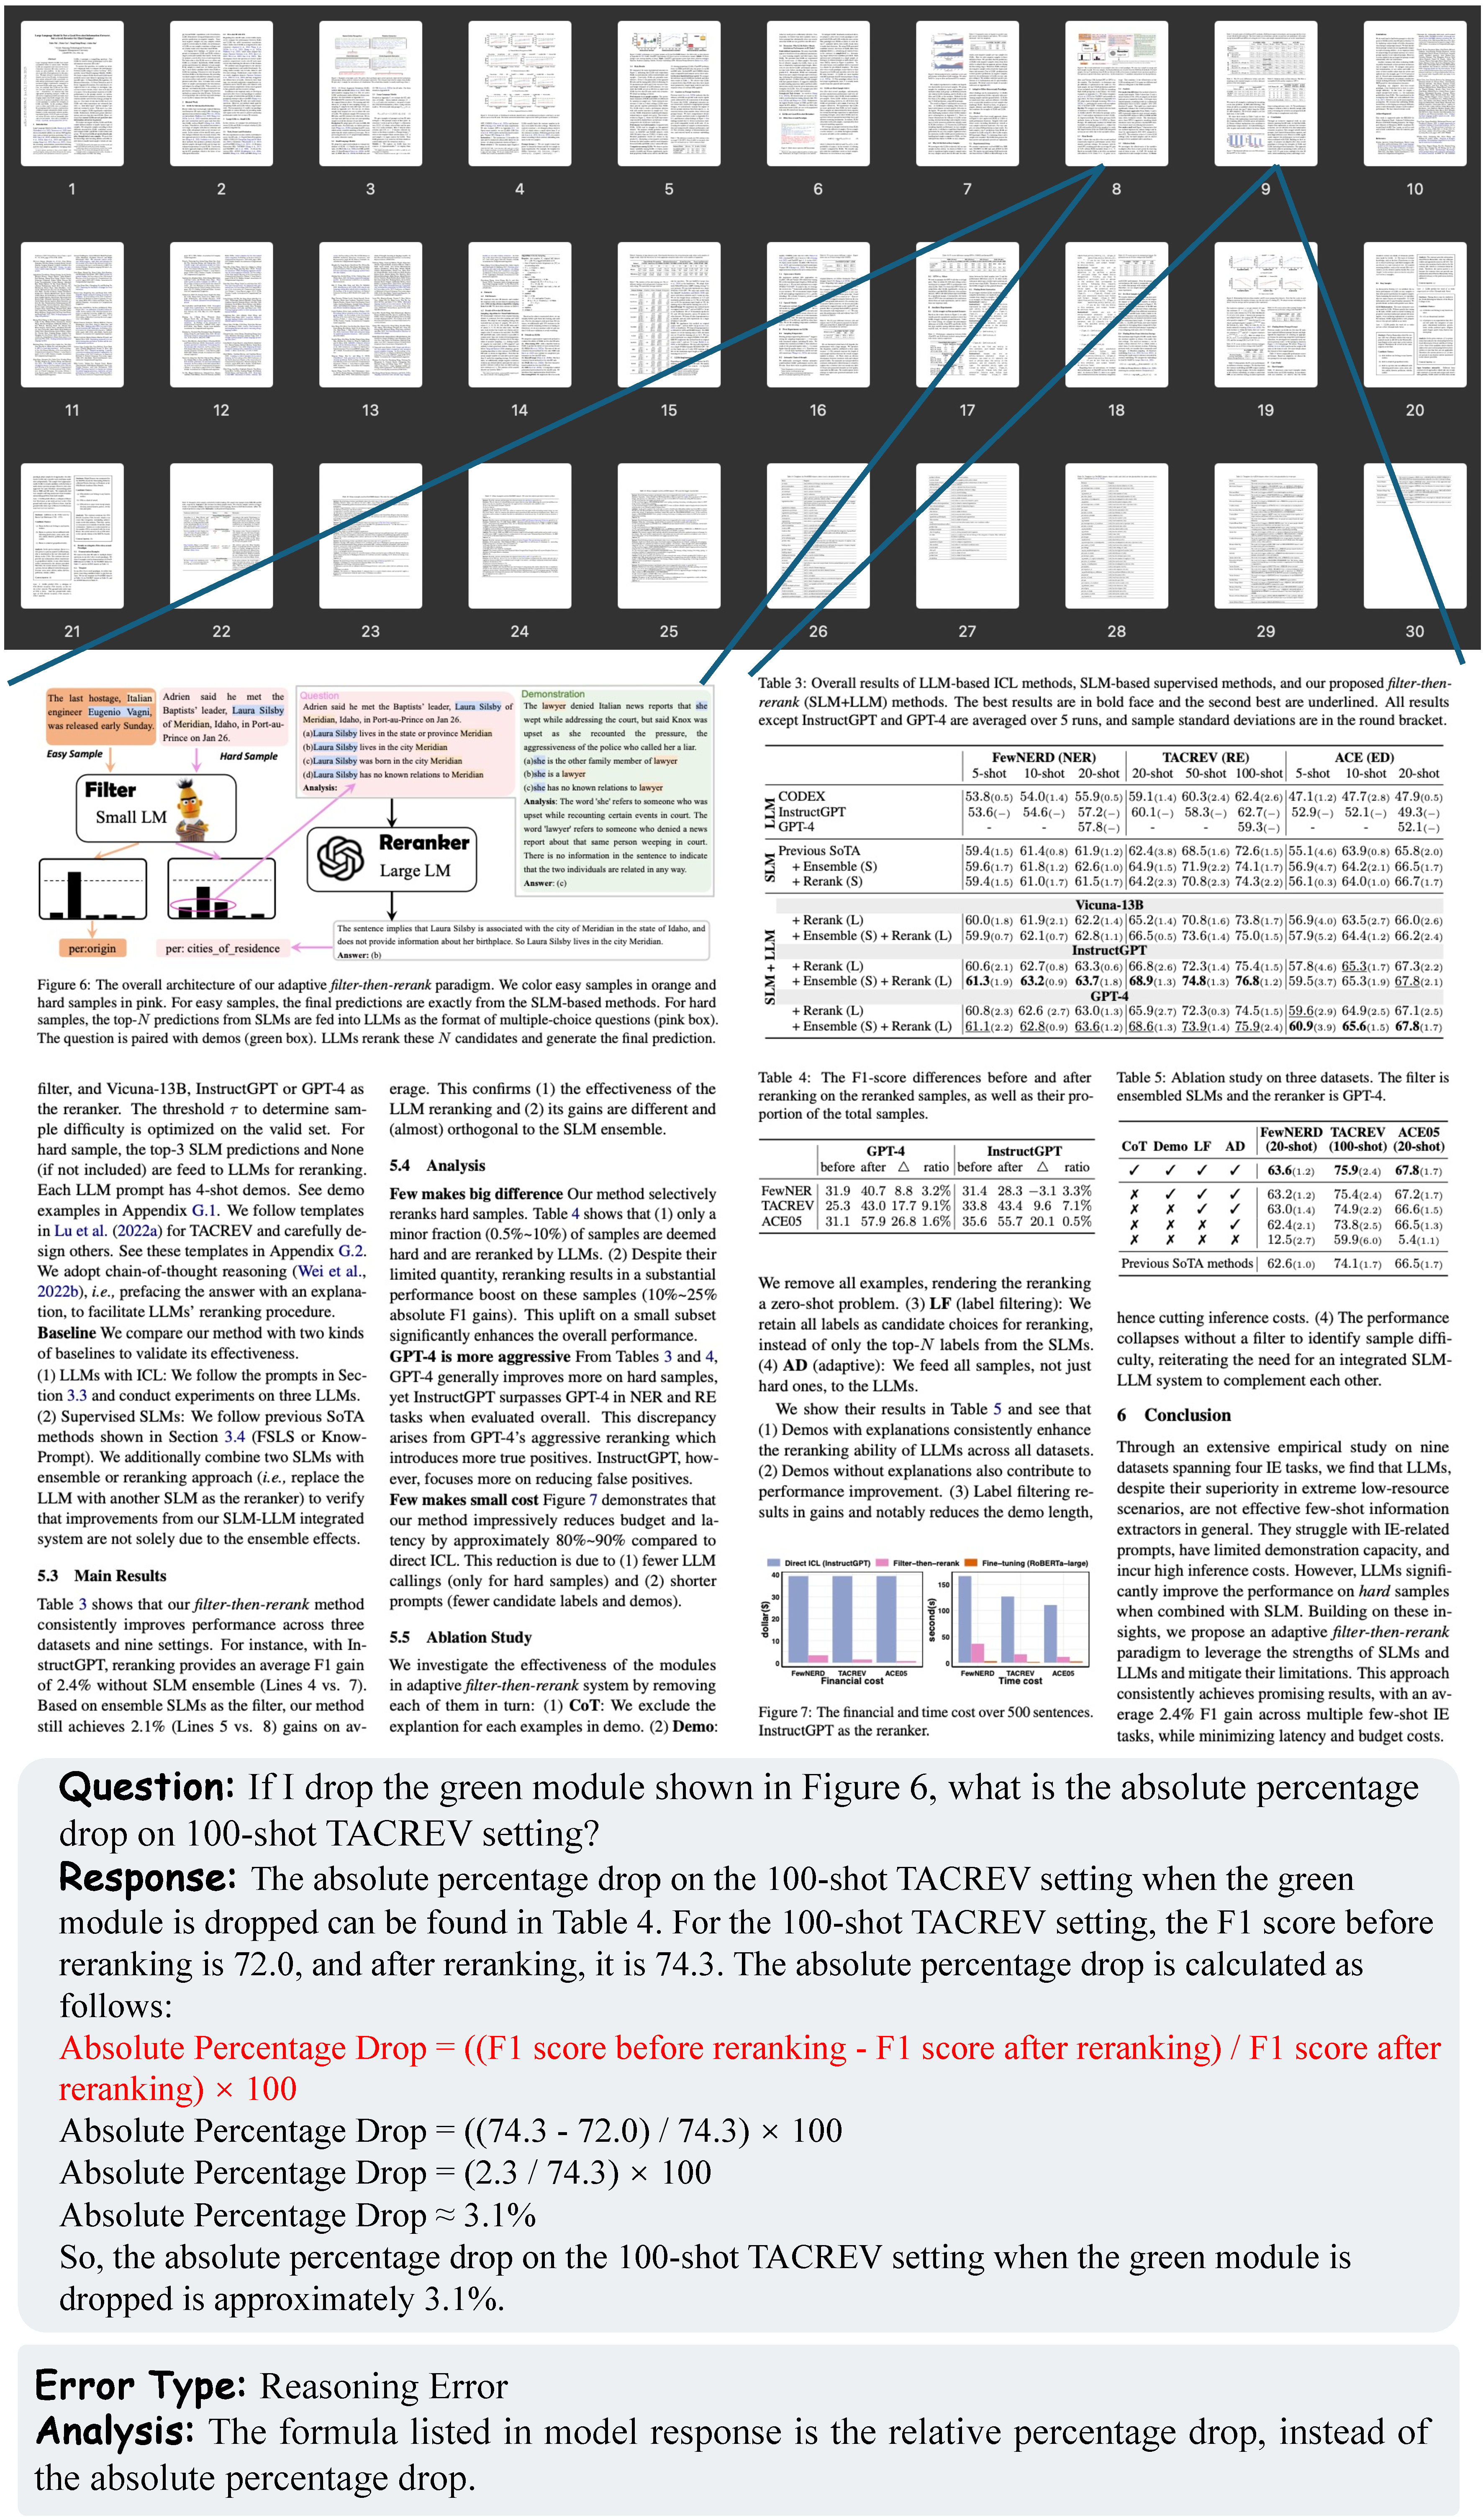
\includegraphics[width=0.85\linewidth]{figures/reasoning_error.pdf}
    \caption{Error example about \textit{Reasoning Error}}
    \label{fig: reasoning_error_1}
\end{figure}

\clearpage
\noindent\textbf{Reasoning Error: Case 2}
\begin{figure}[!htbp]
    \centering
    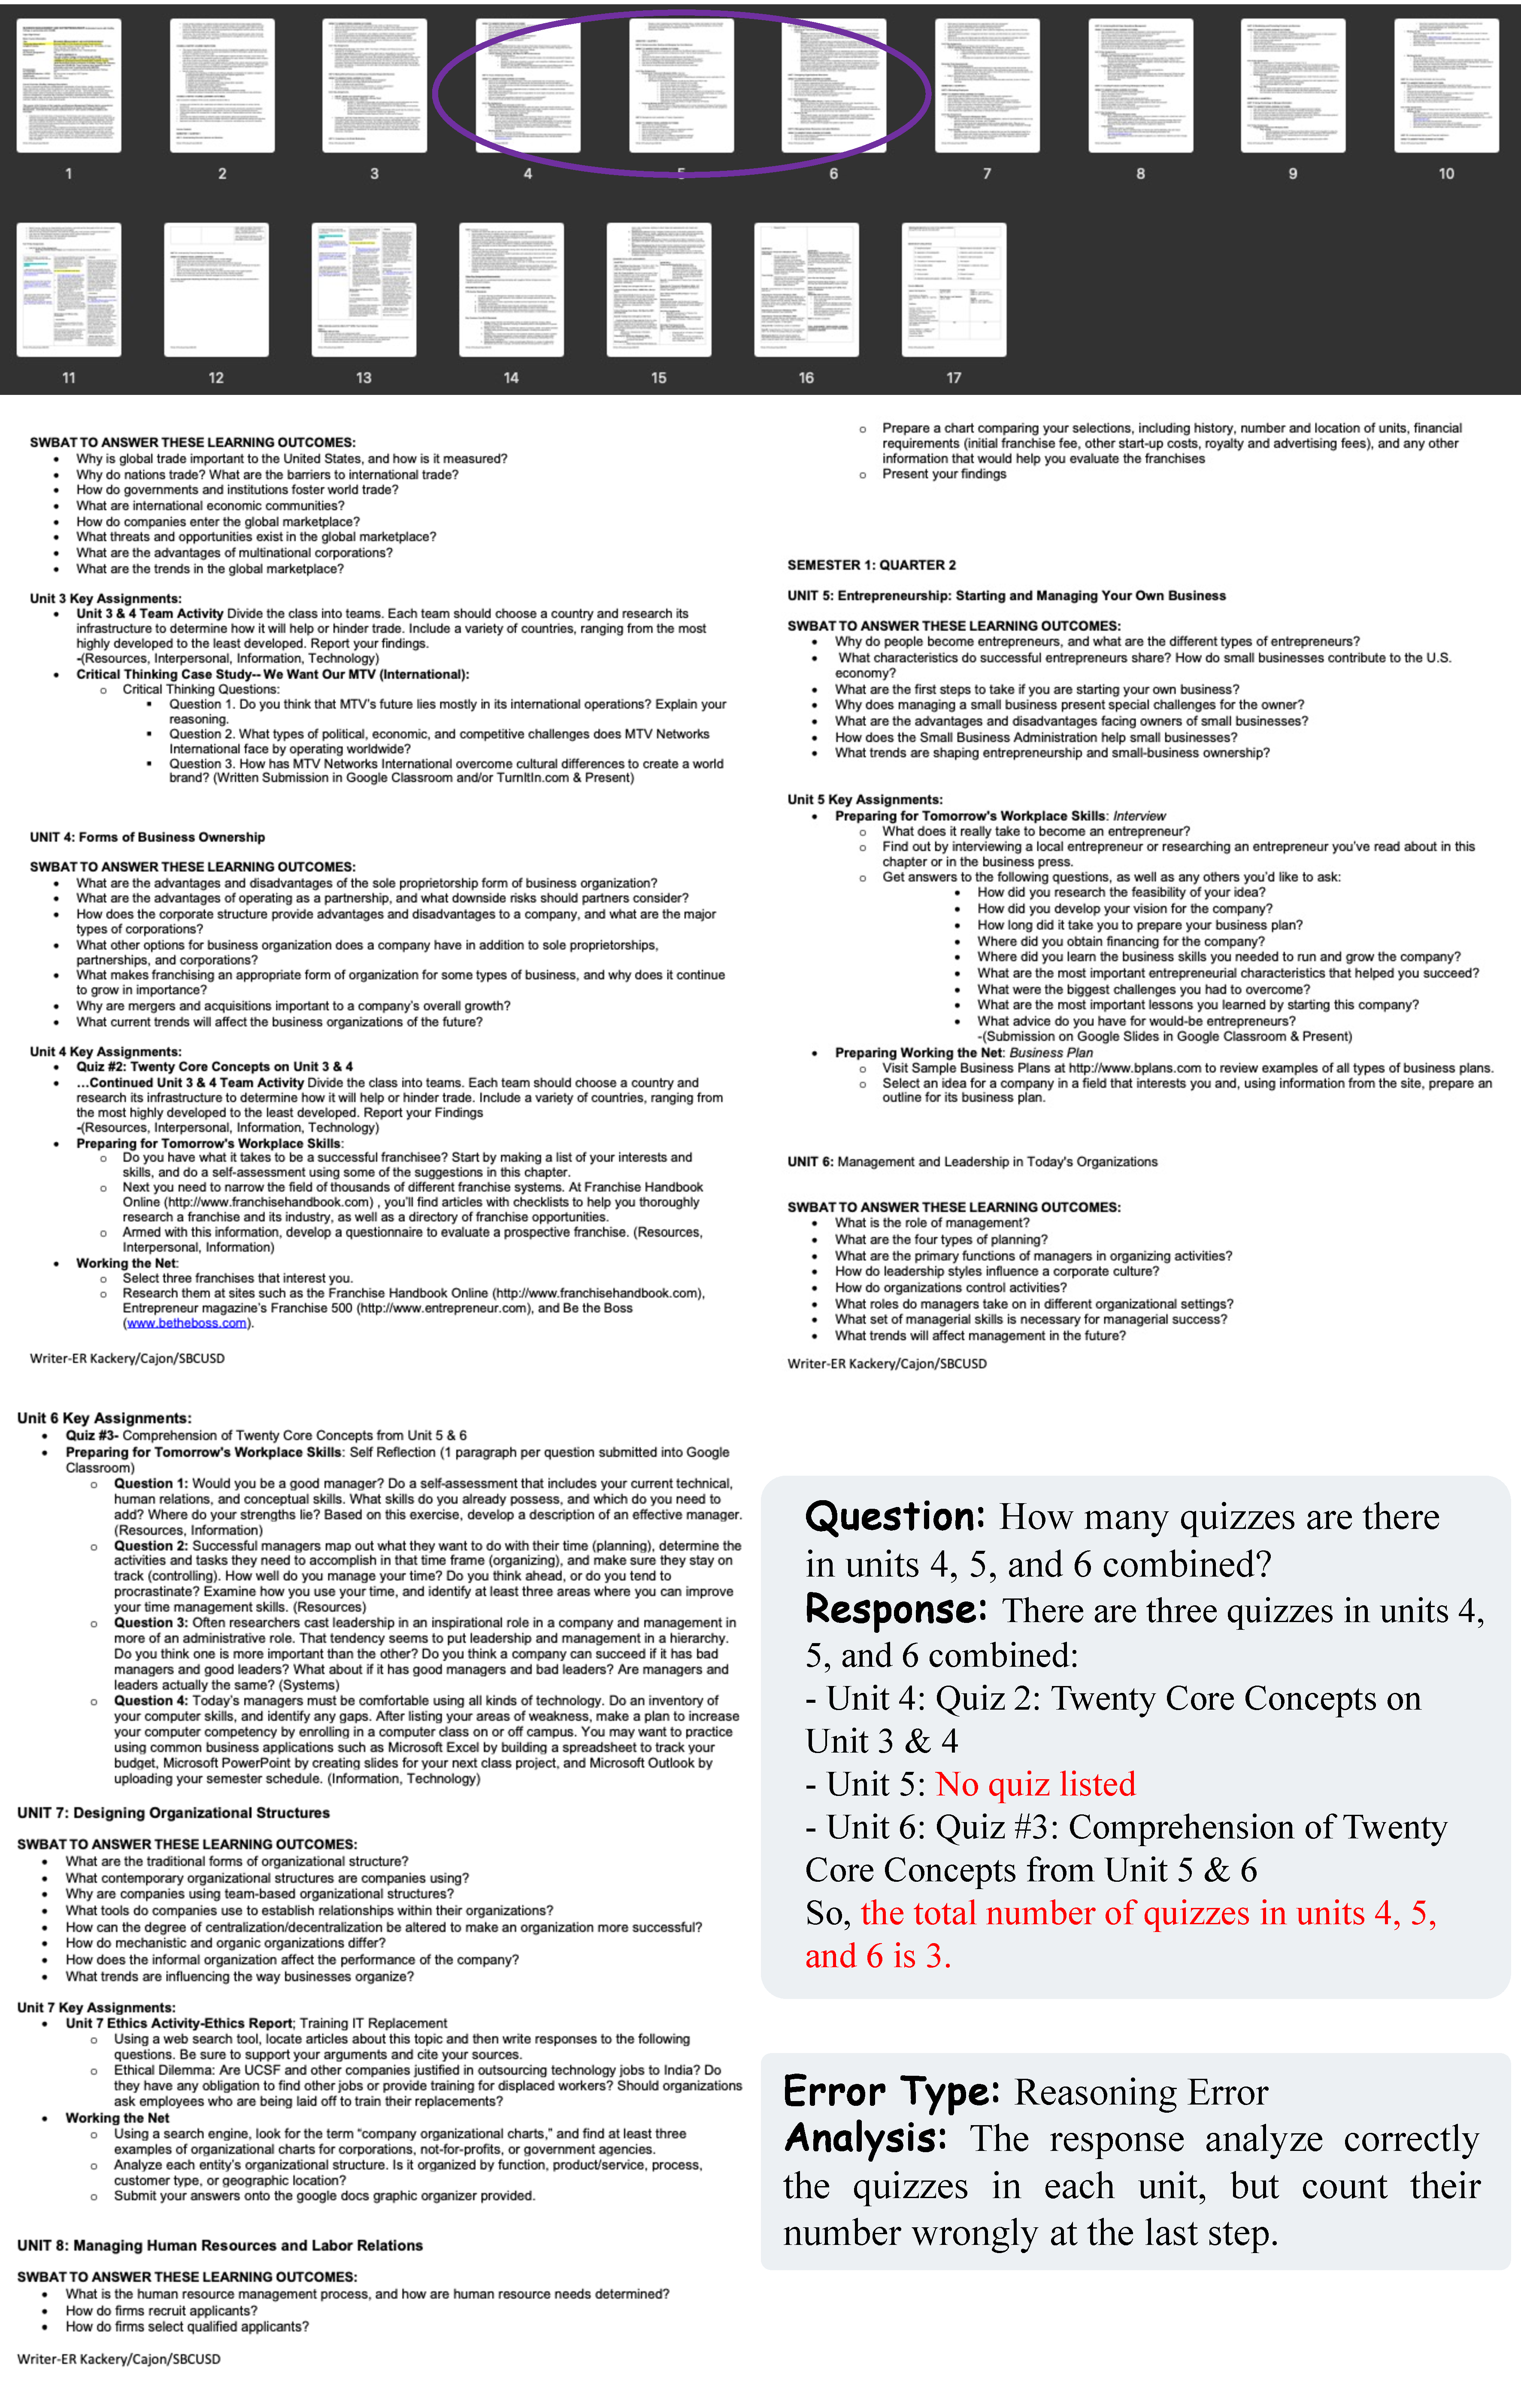
\includegraphics[width=0.9\linewidth]{figures/Reasoning_error_2.pdf}
    \caption{Error example about \textit{Reasoning Error}}
    \label{fig: reasoning_error_2}
\end{figure}

\clearpage
\noindent\textbf{Irrelevant Answer: Case 1}
\begin{figure}[!htbp]
    \centering
    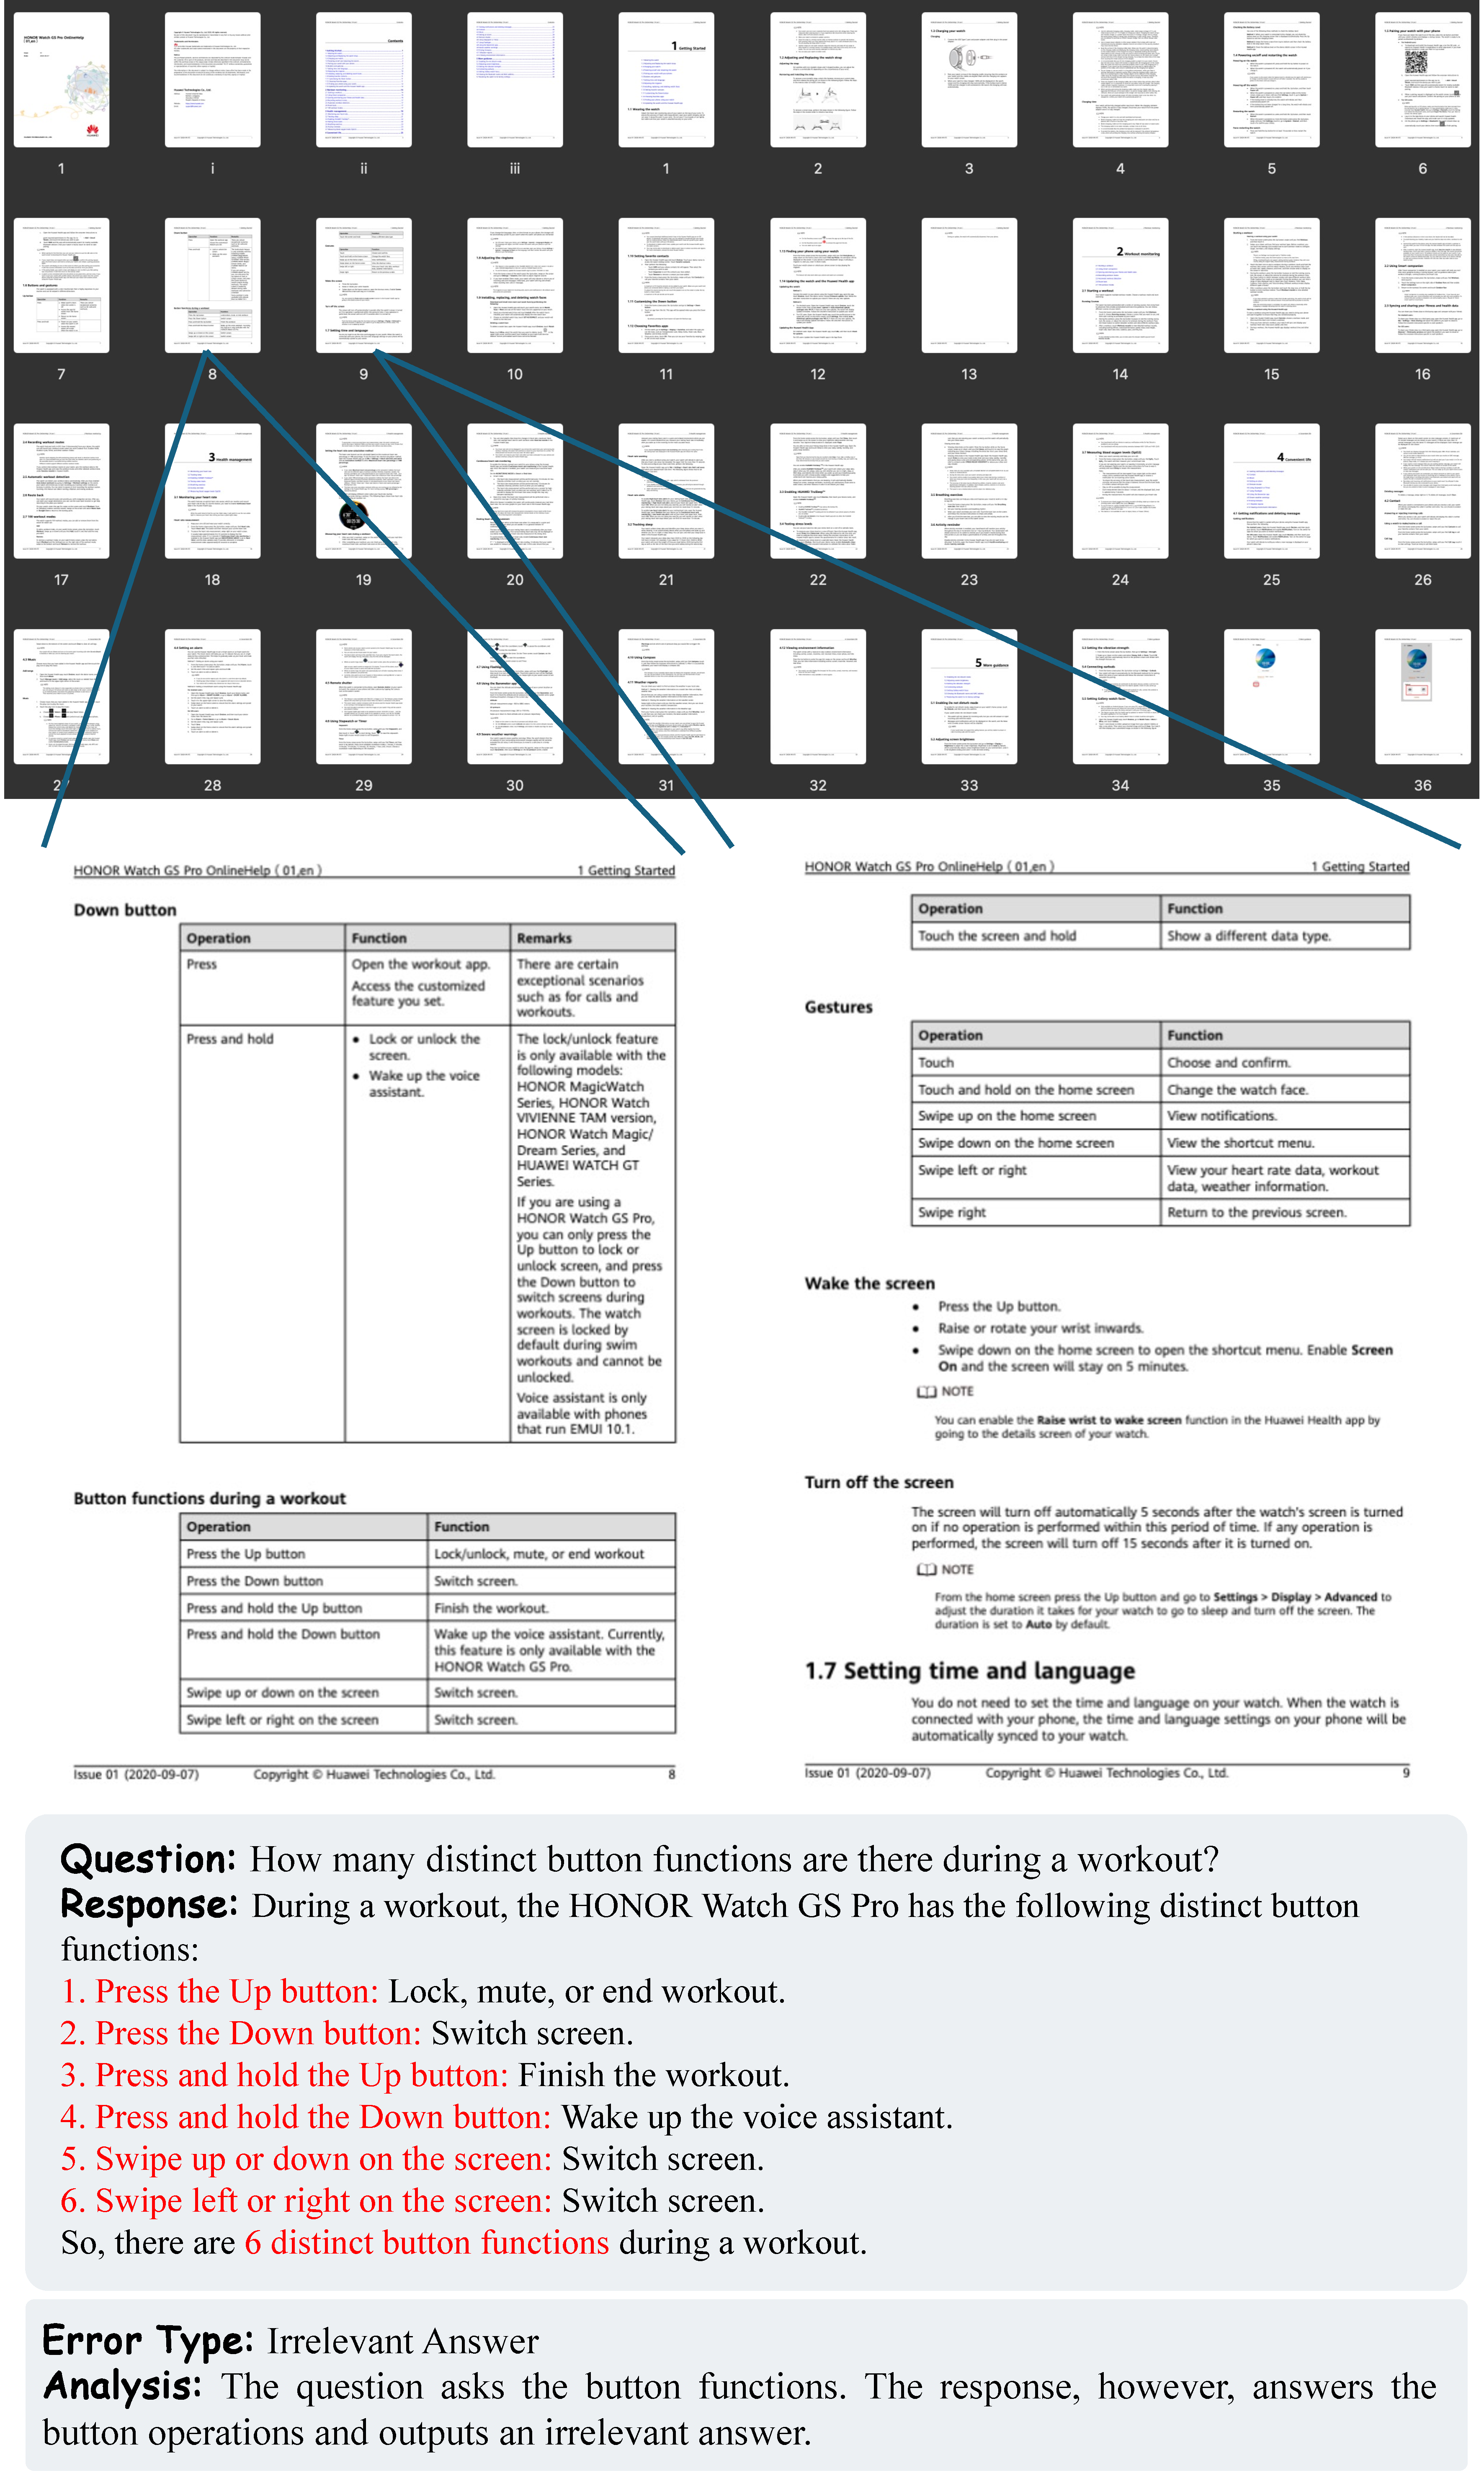
\includegraphics[width=0.85\linewidth]{figures/Irrelevant_answer.pdf}
    \caption{Error example about \textit{Irrelevant Answer}}
    \label{fig: irrelevant_answer_1}
\end{figure}

\clearpage
\noindent\textbf{Irrelevant Answer: Case 2}
\begin{figure}[!htbp]
    \centering
    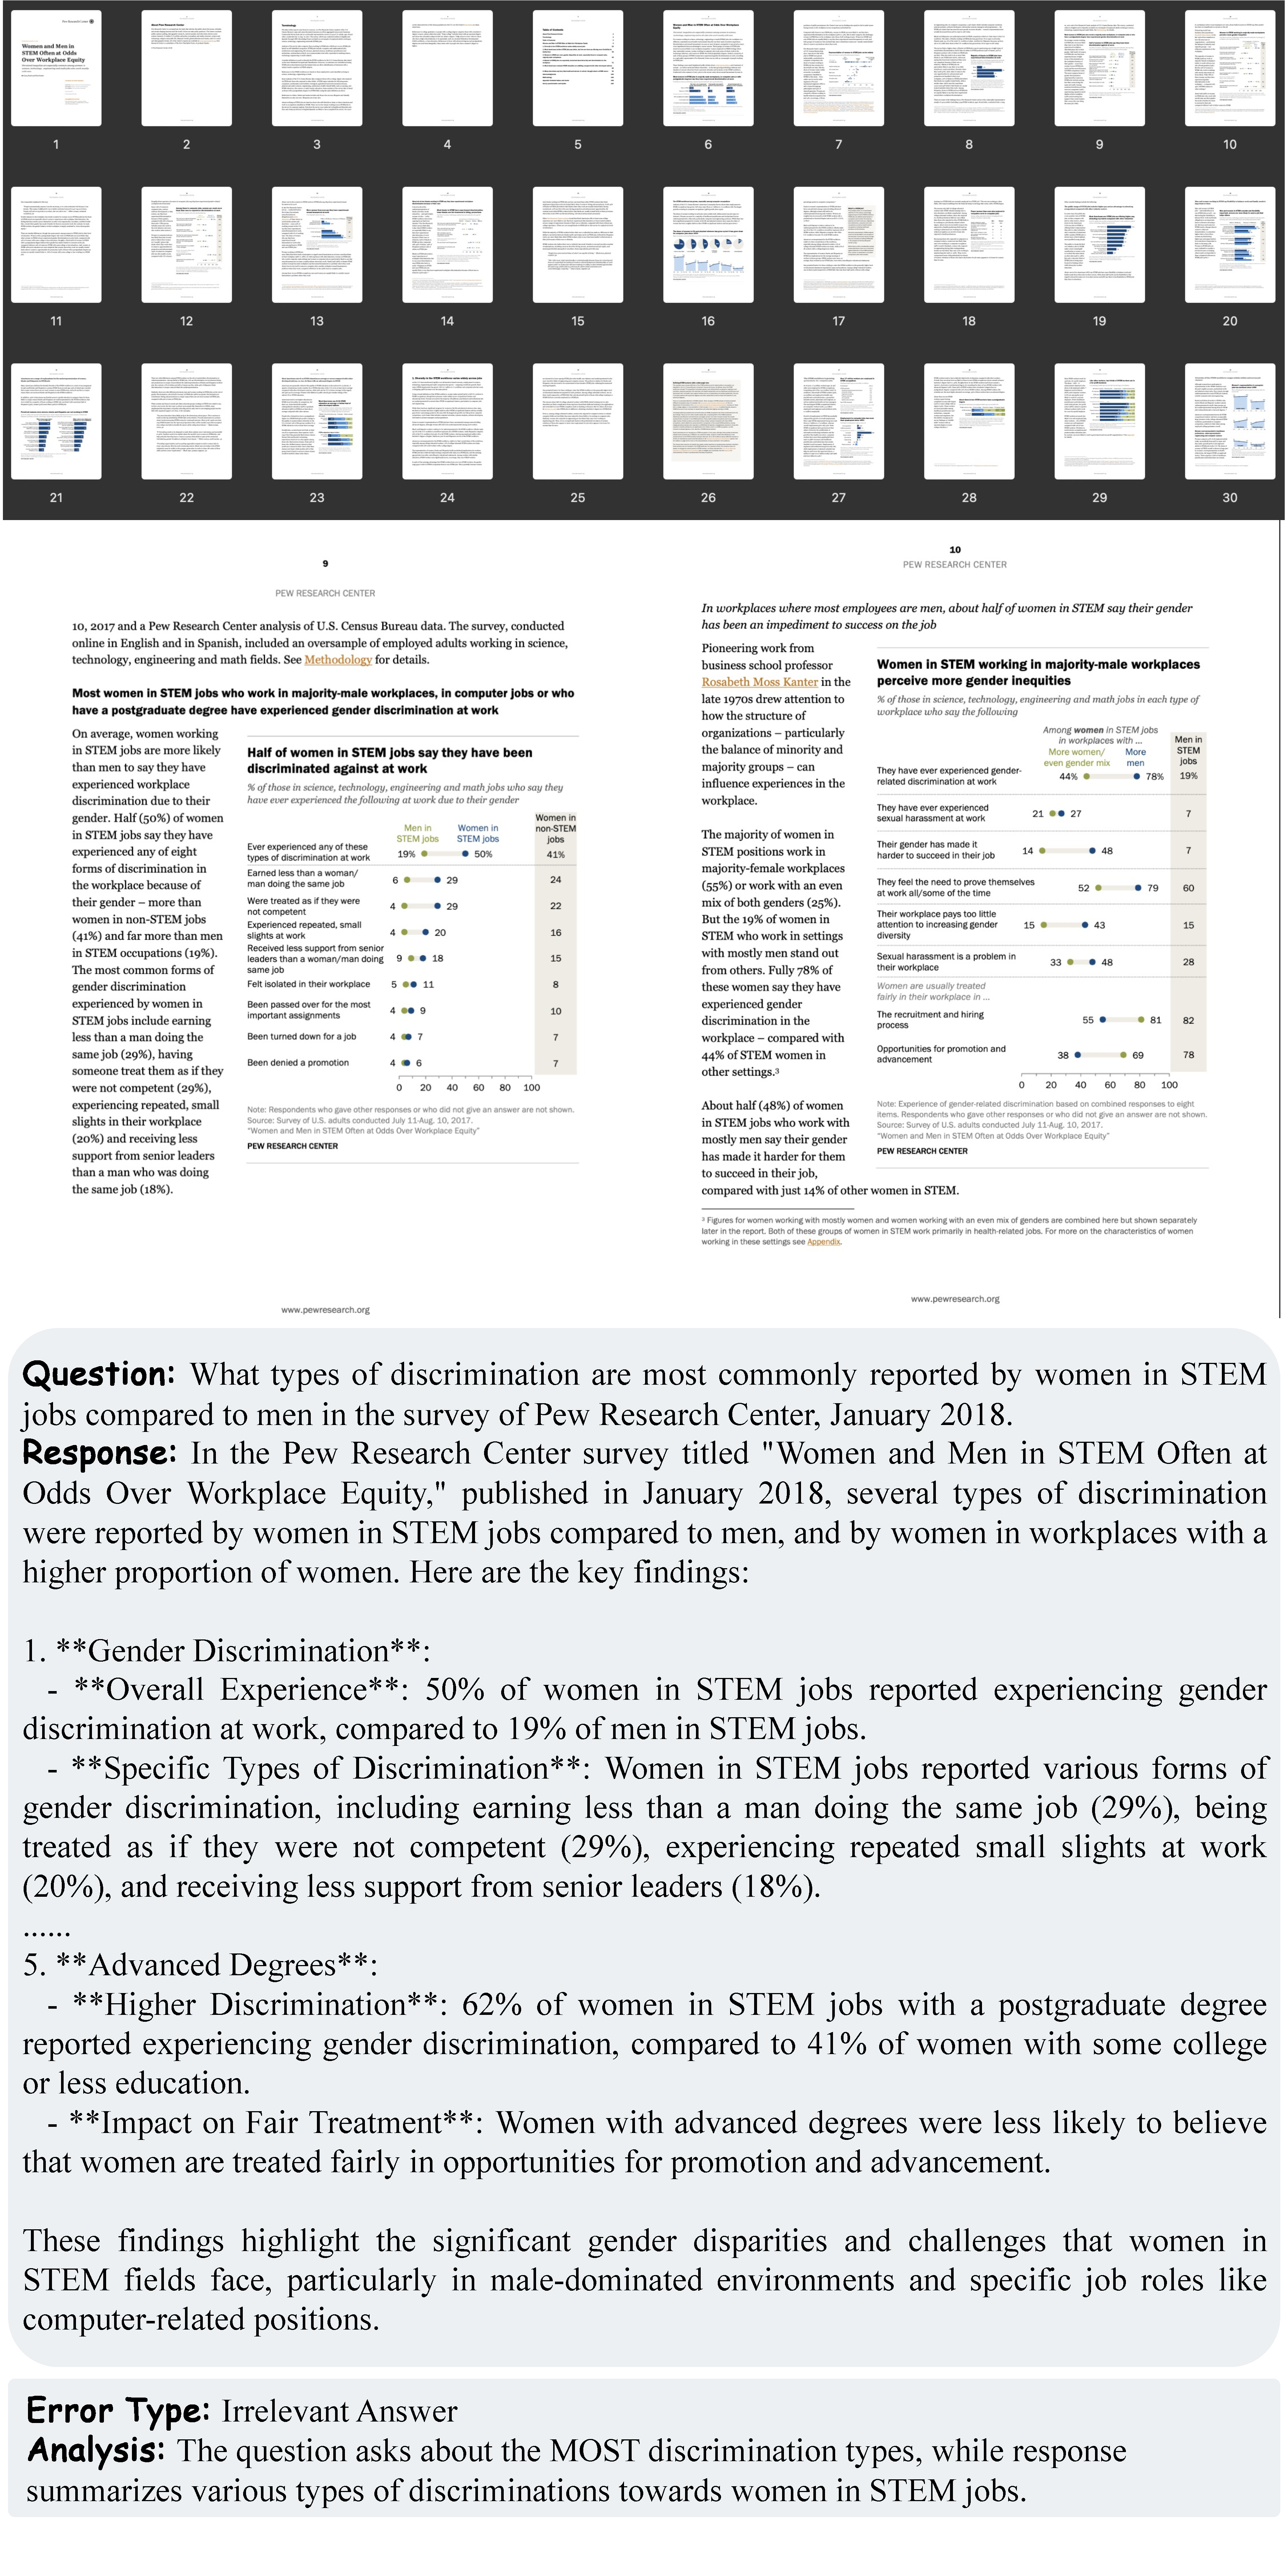
\includegraphics[width=0.75\linewidth]{figures/Irrevelant_answer_2.pdf}
    \caption{Error example about \textit{Irrelevant Answer}}
    \label{fig: irrelevant_answer_2}
\end{figure}


\subsection{Case Study}
\label{appendix: case_study}

\begin{figure}[!htbp]
    \centering
    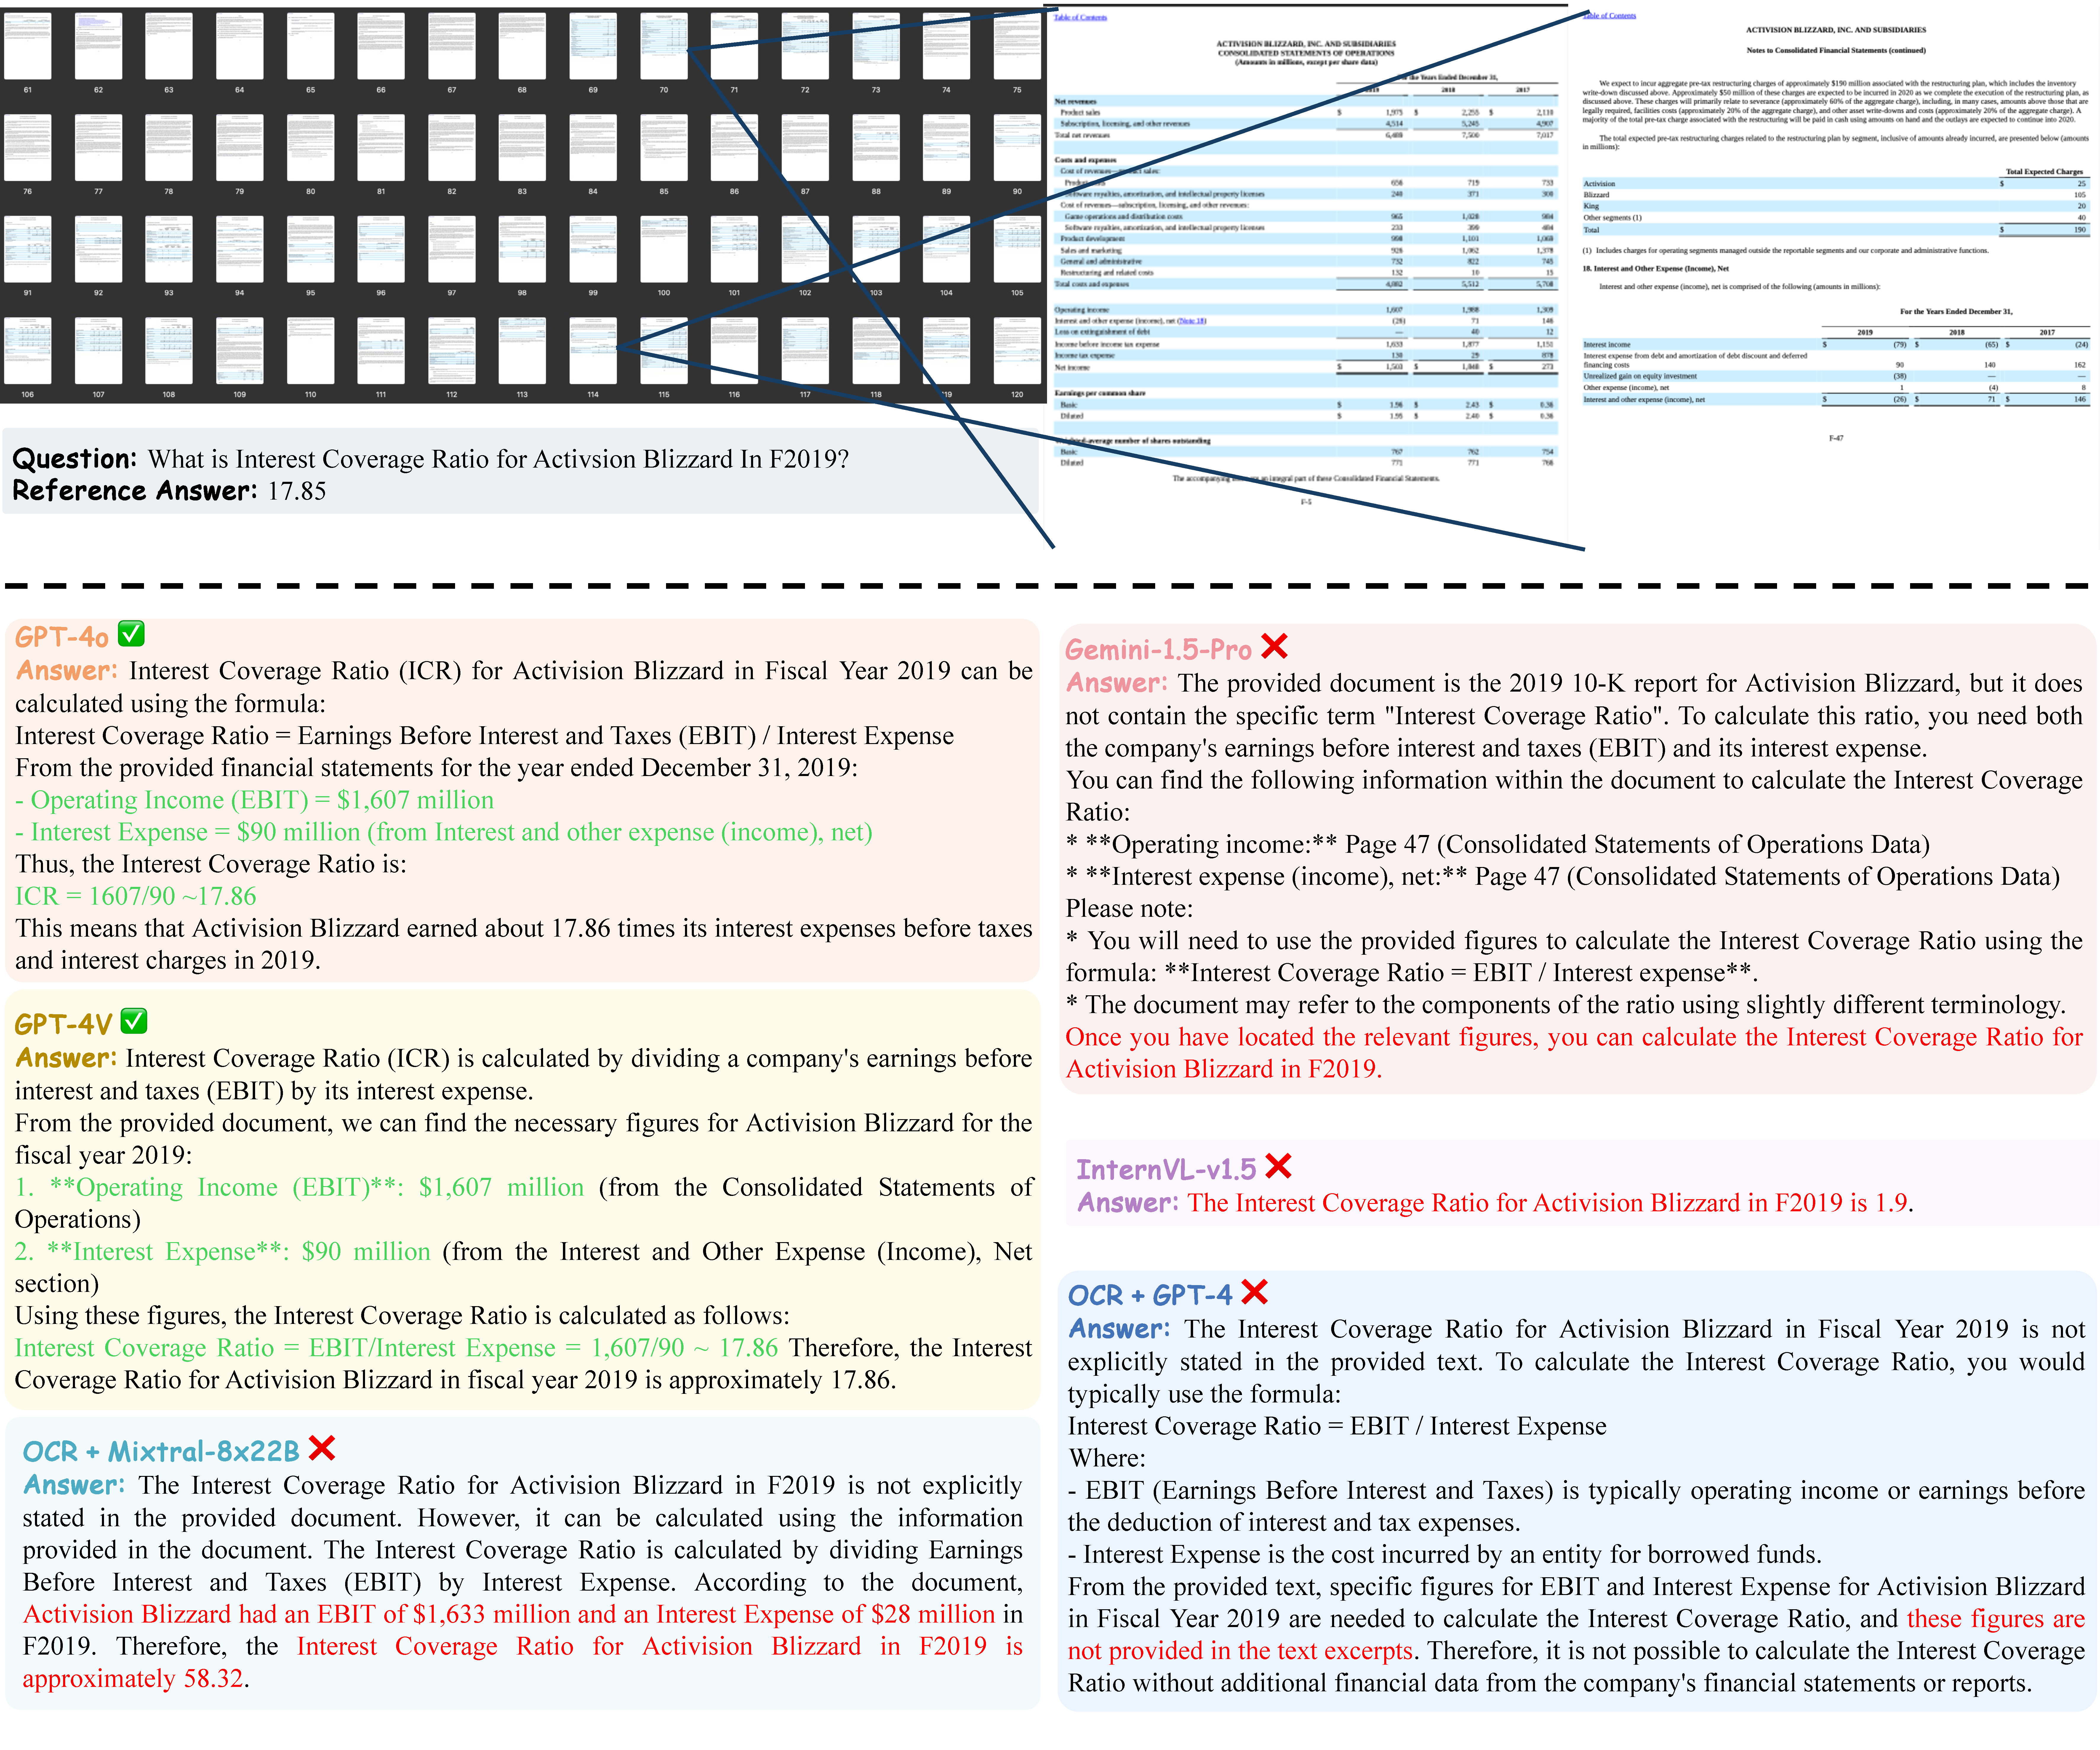
\includegraphics[width=0.95\linewidth]{figures/table_1.pdf}
    \caption{Case Study. Evidence source: table. The evidence pages are zoomed in. The correct extracted information and reasoning are colored in green, and the wrong ones are colored in red.}
    \label{fig: case_3}
\end{figure}

\clearpage
\begin{figure}
    \centering
    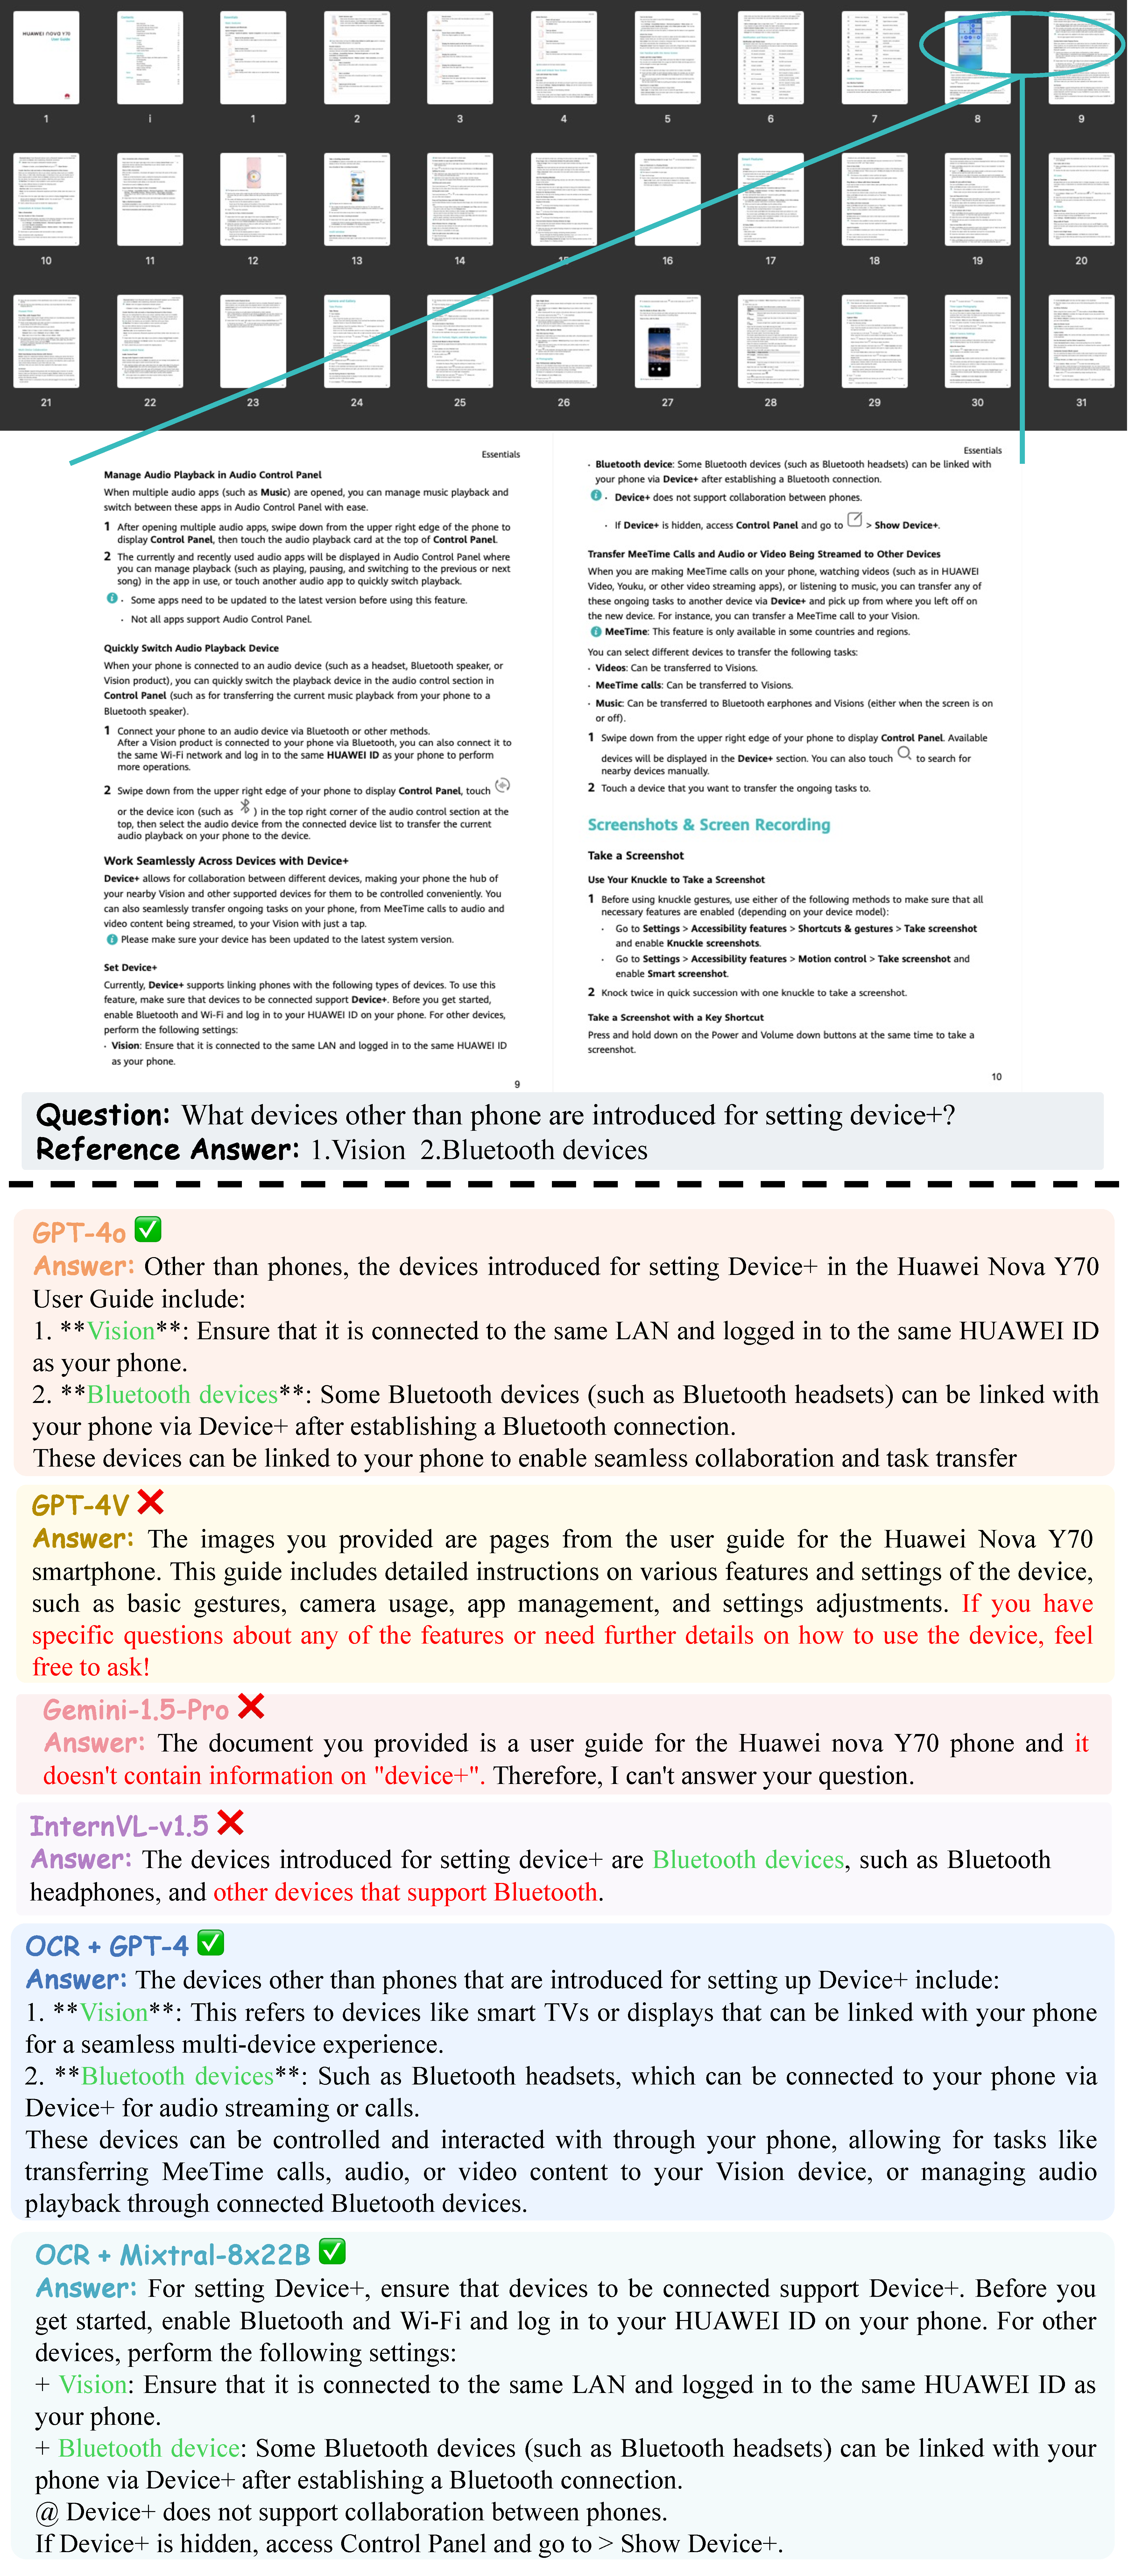
\includegraphics[width=0.7\linewidth]{figures/text_1.pdf}
    \caption{Case Study. Evidence source: text. The evidence pages are zoomed in. The correct extracted information and reasoning are colored in green, and the wrong ones are colored in red.}
    \label{fig: case_4}
\end{figure}

\clearpage
\begin{figure}
    \centering
    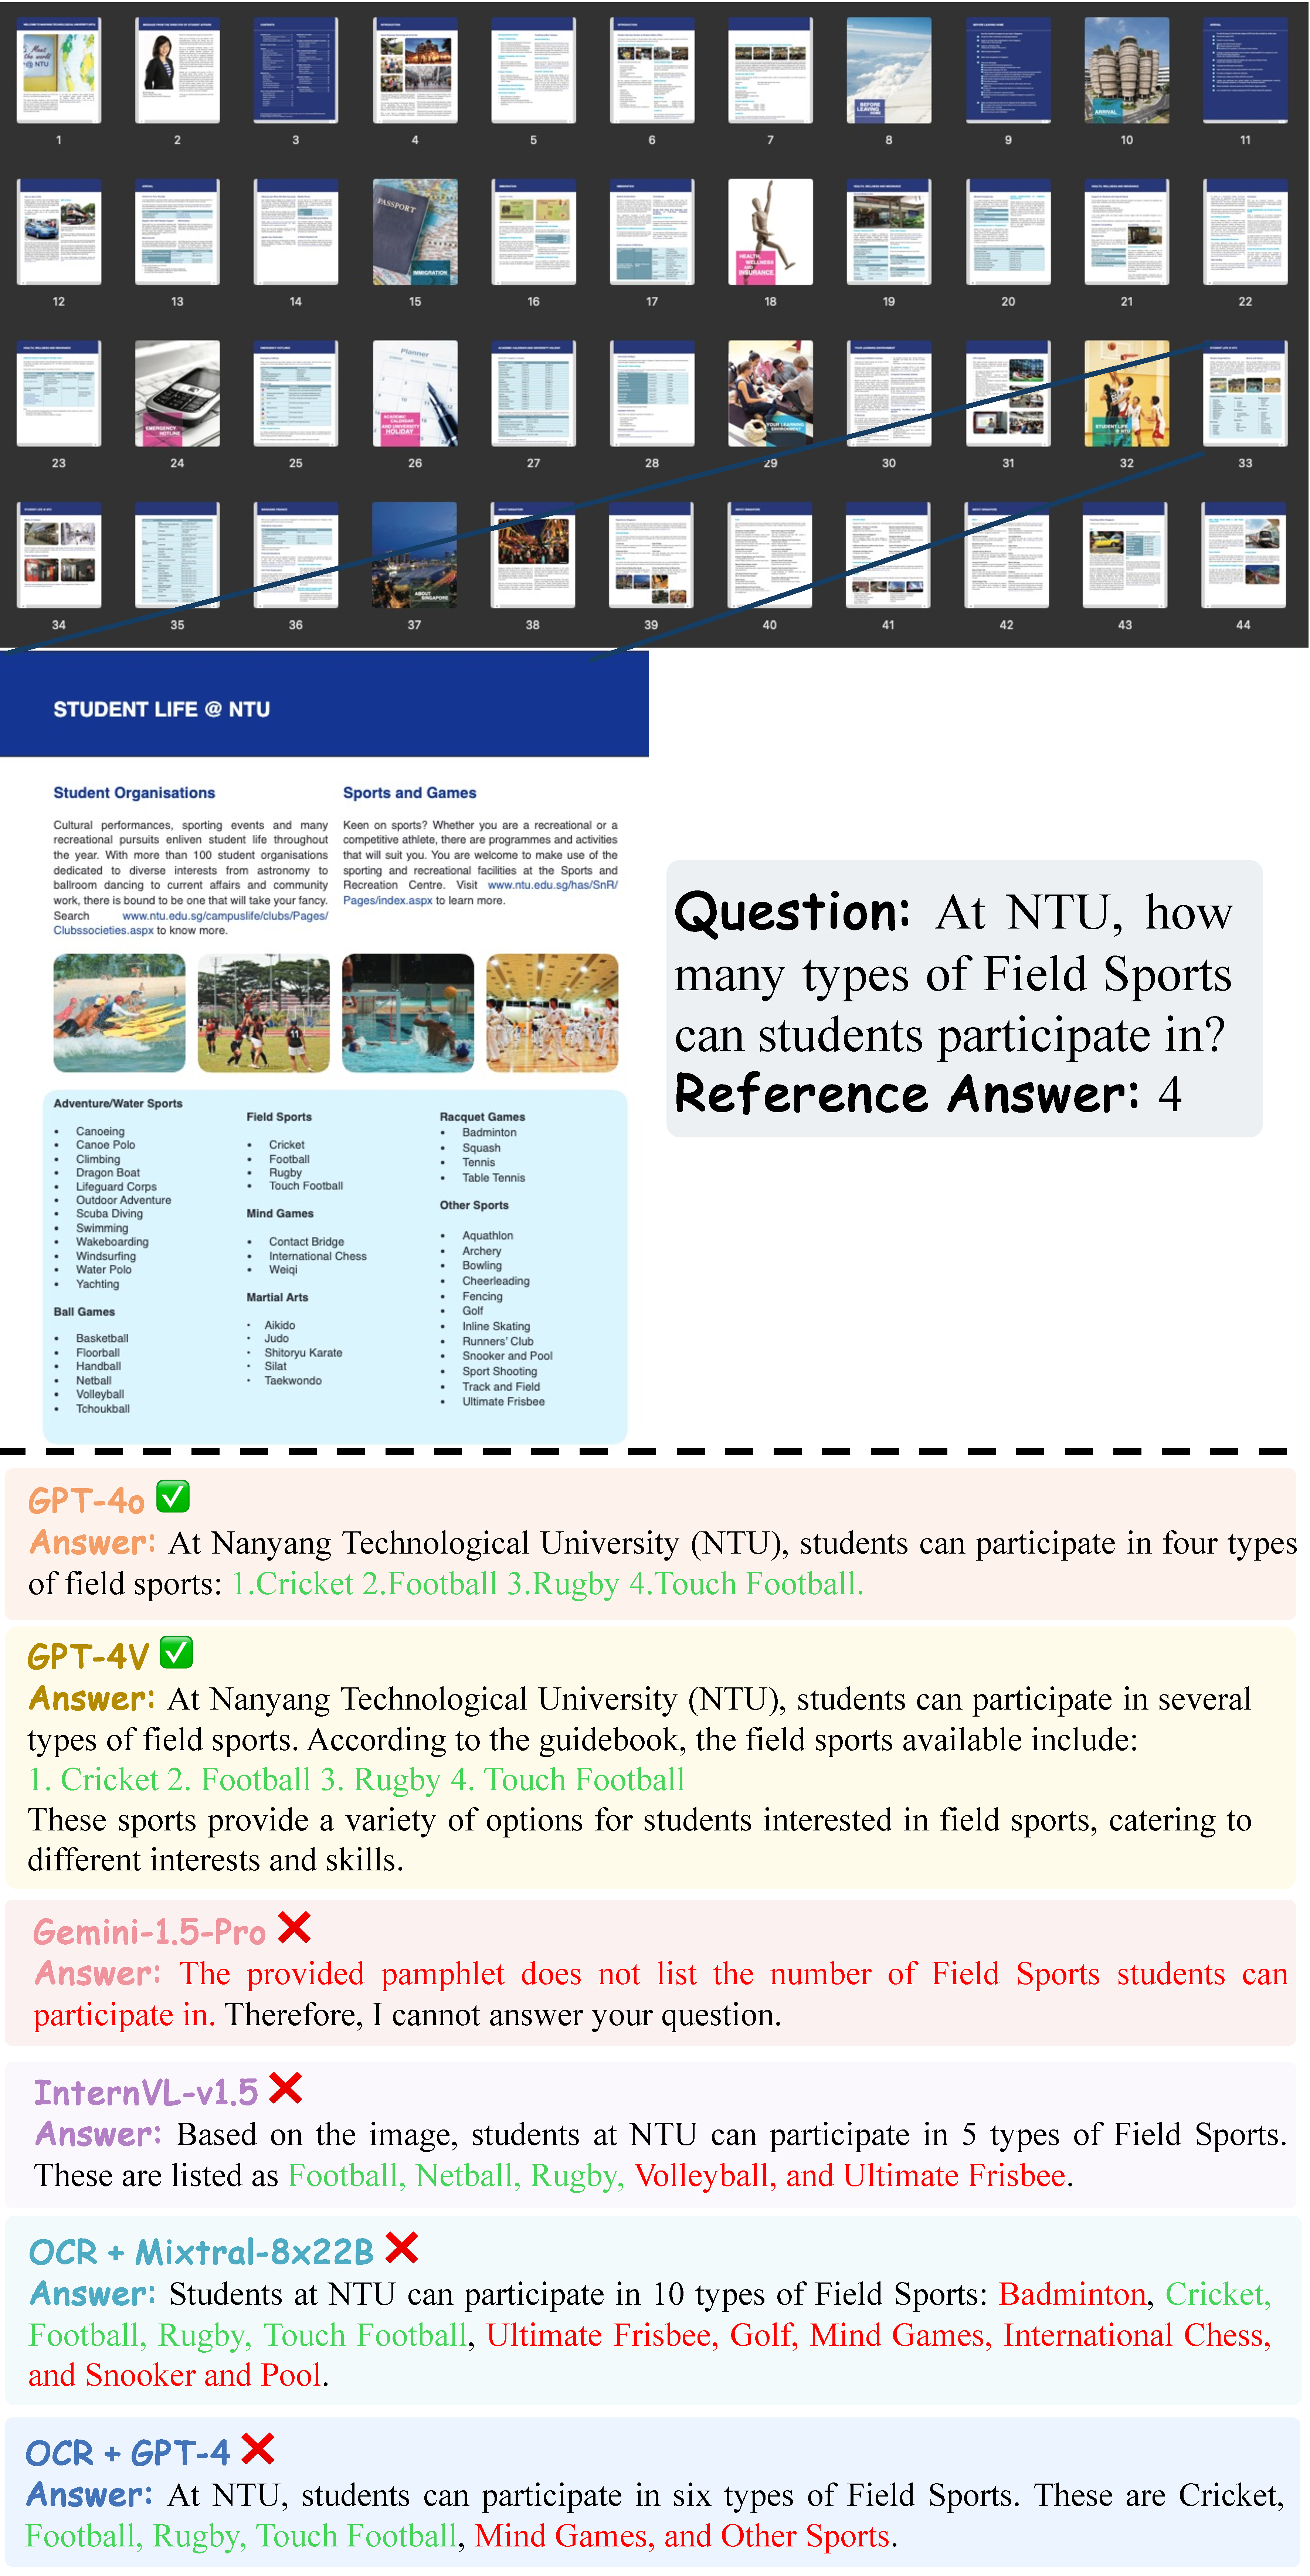
\includegraphics[width=0.7\linewidth]{figures/layout_1.pdf}
    \caption{Case Study. Evidence source: layout. The evidence page is zoomed in. The correct extracted information and reasoning are colored in green, and the wrong ones are colored in red.}
    \label{fig: case_5}
\end{figure}

\begin{figure}[!b]
    \centering
    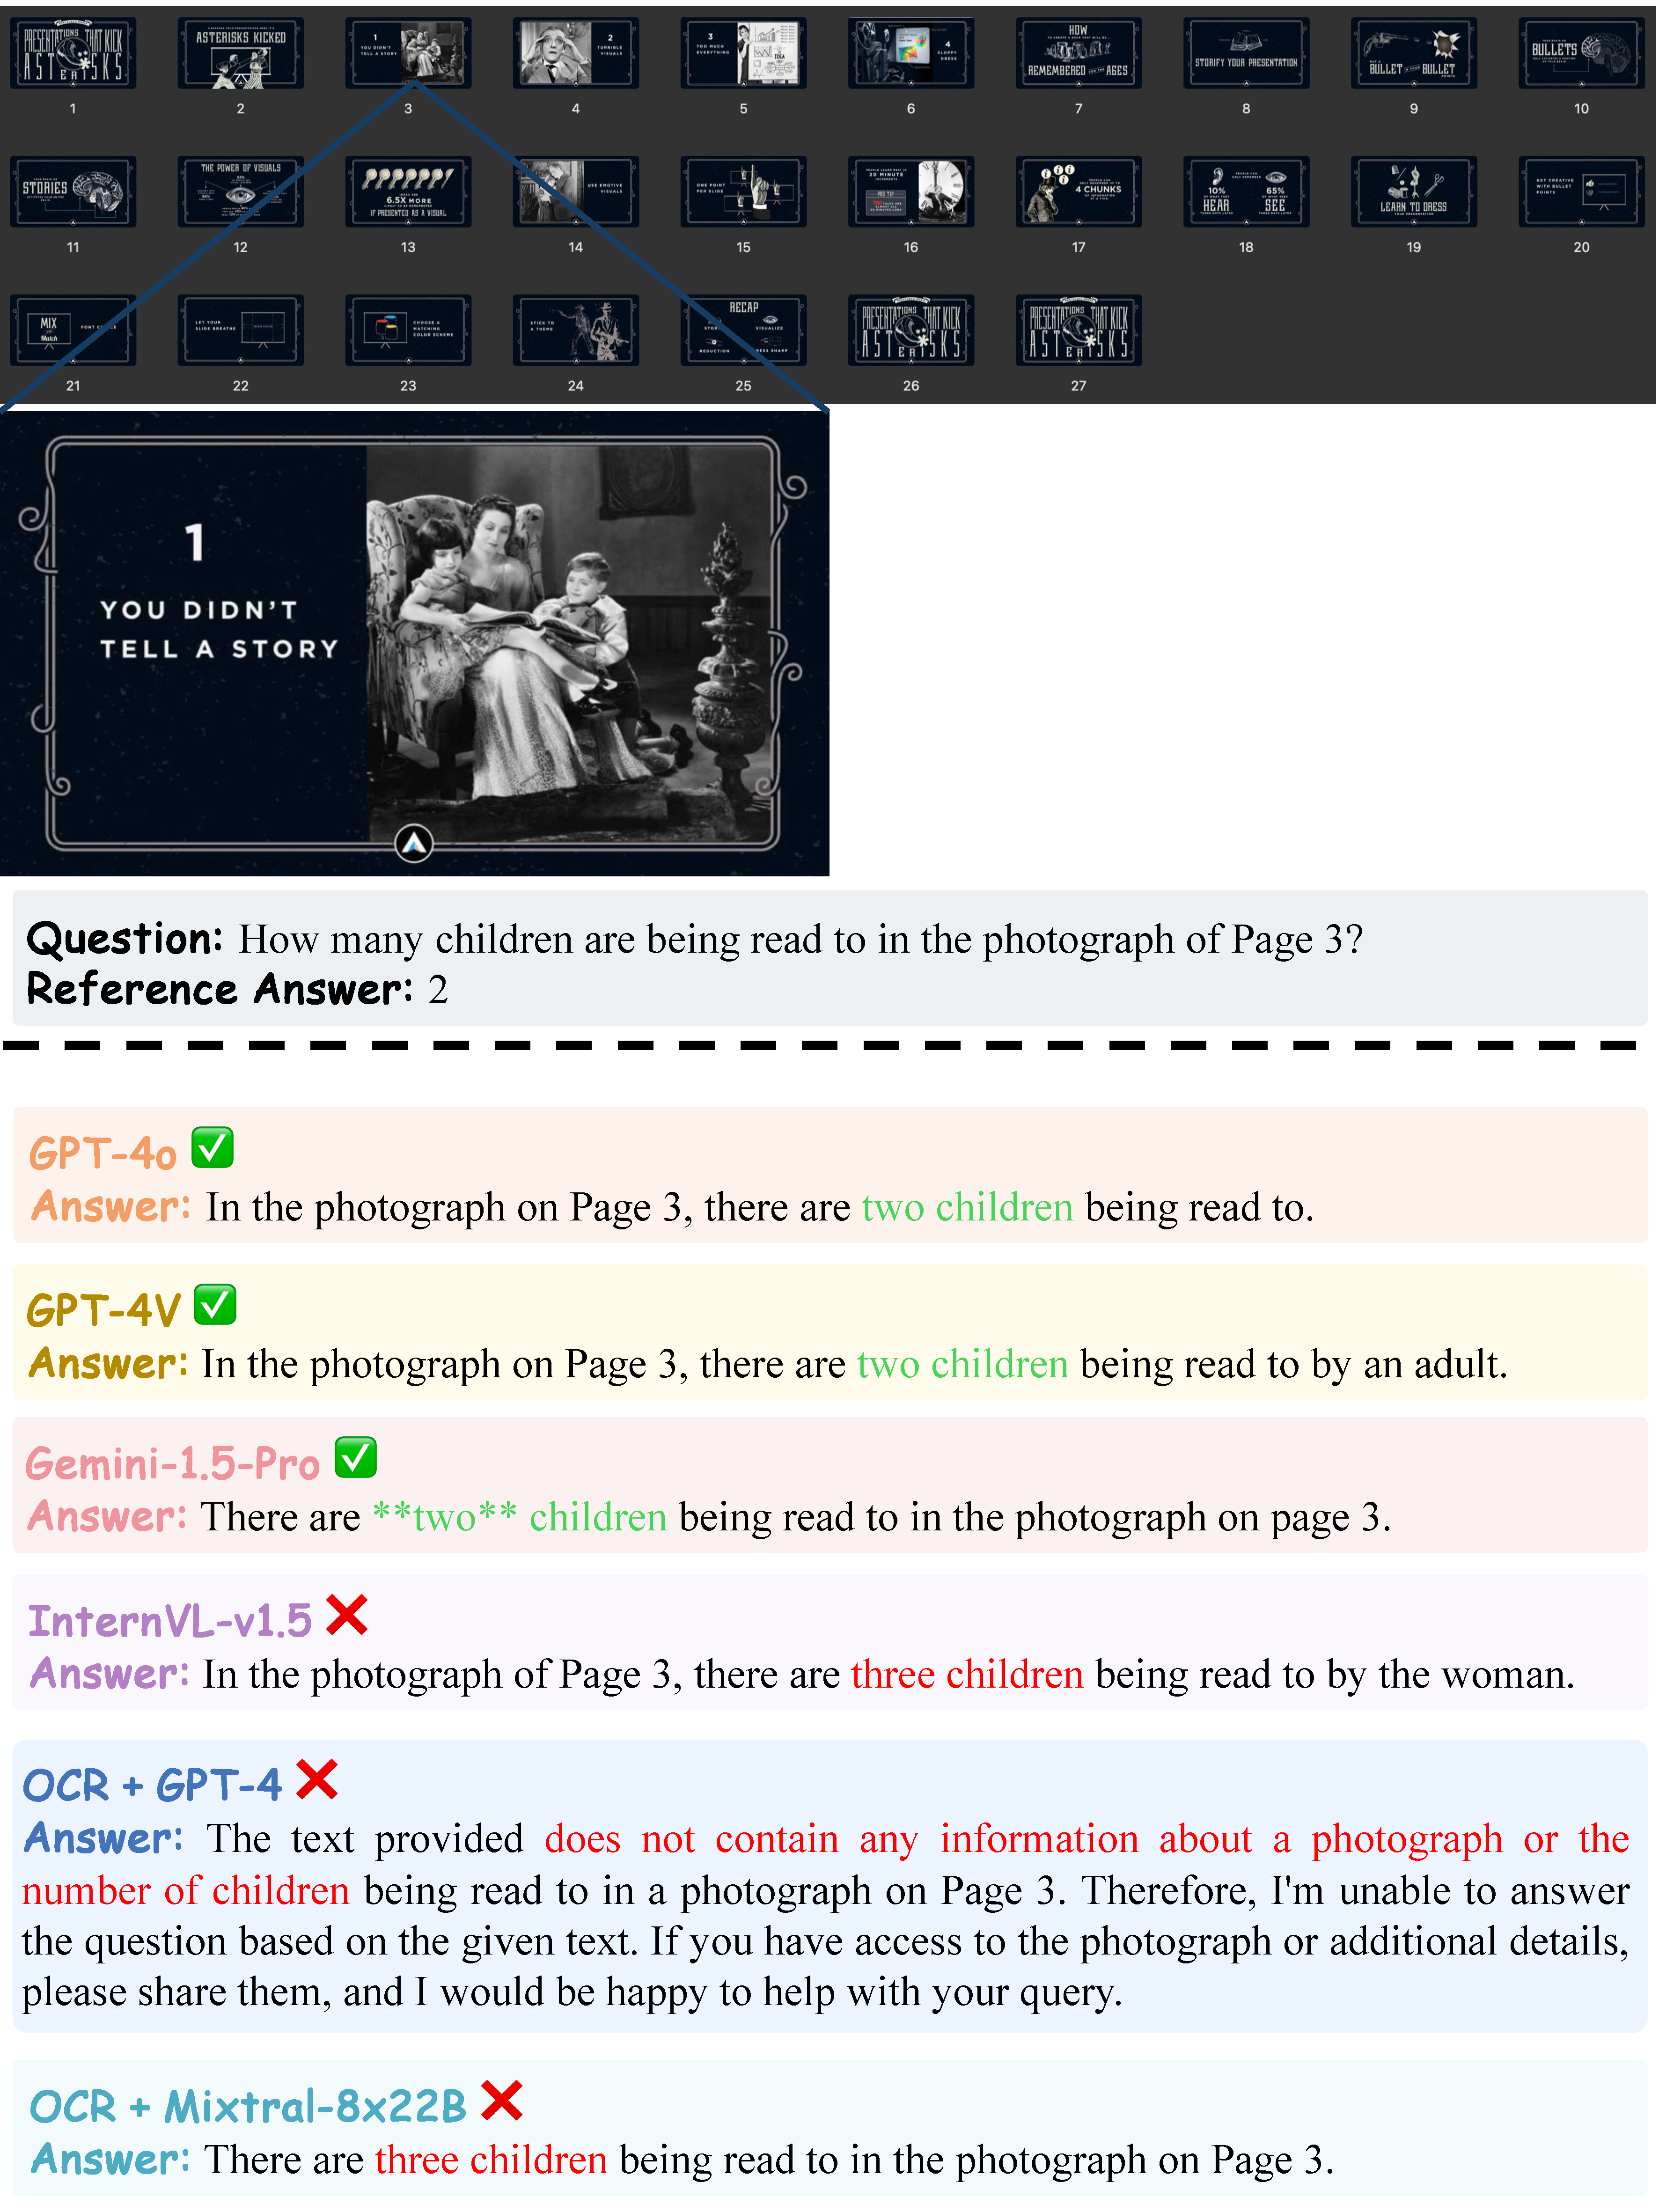
\includegraphics[width=0.7\linewidth]{figures/image_1.pdf}
    \caption{Case Study. Evidence source: image. The evidence page is zoomed in. The correct extracted information and reasoning are colored in green, and the wrong ones are colored in red.}
    \label{fig: case_1}
\end{figure}
